\chapter{Entrevistas con Metodología de la Metáfora}
\label{ch:anexo-a}
\newpage
%\blindtext[5]
\underline {ENTREVISTA 1} \\
Nombre: Marcel\\
Edad: 25\\
Carrera: 4to Año de Ingeniería Civil Informática y Telecomunicaciones\\
Comuna: Santiago Centro \\

\begin{longtable}{>{\centering\arraybackslash}m{1cm} >{\centering\arraybackslash}m{2cm} >{\arraybackslash}m{5cm}>{\arraybackslash}m{5cm}}
	
\hline
Número & Imagen & Descripción & Asociaciones \\
\hline \hline
\endfirsthead

\hline
Número & Imagen & Descripción & Asociaciones \\
\hline \hline
\endhead

1 & 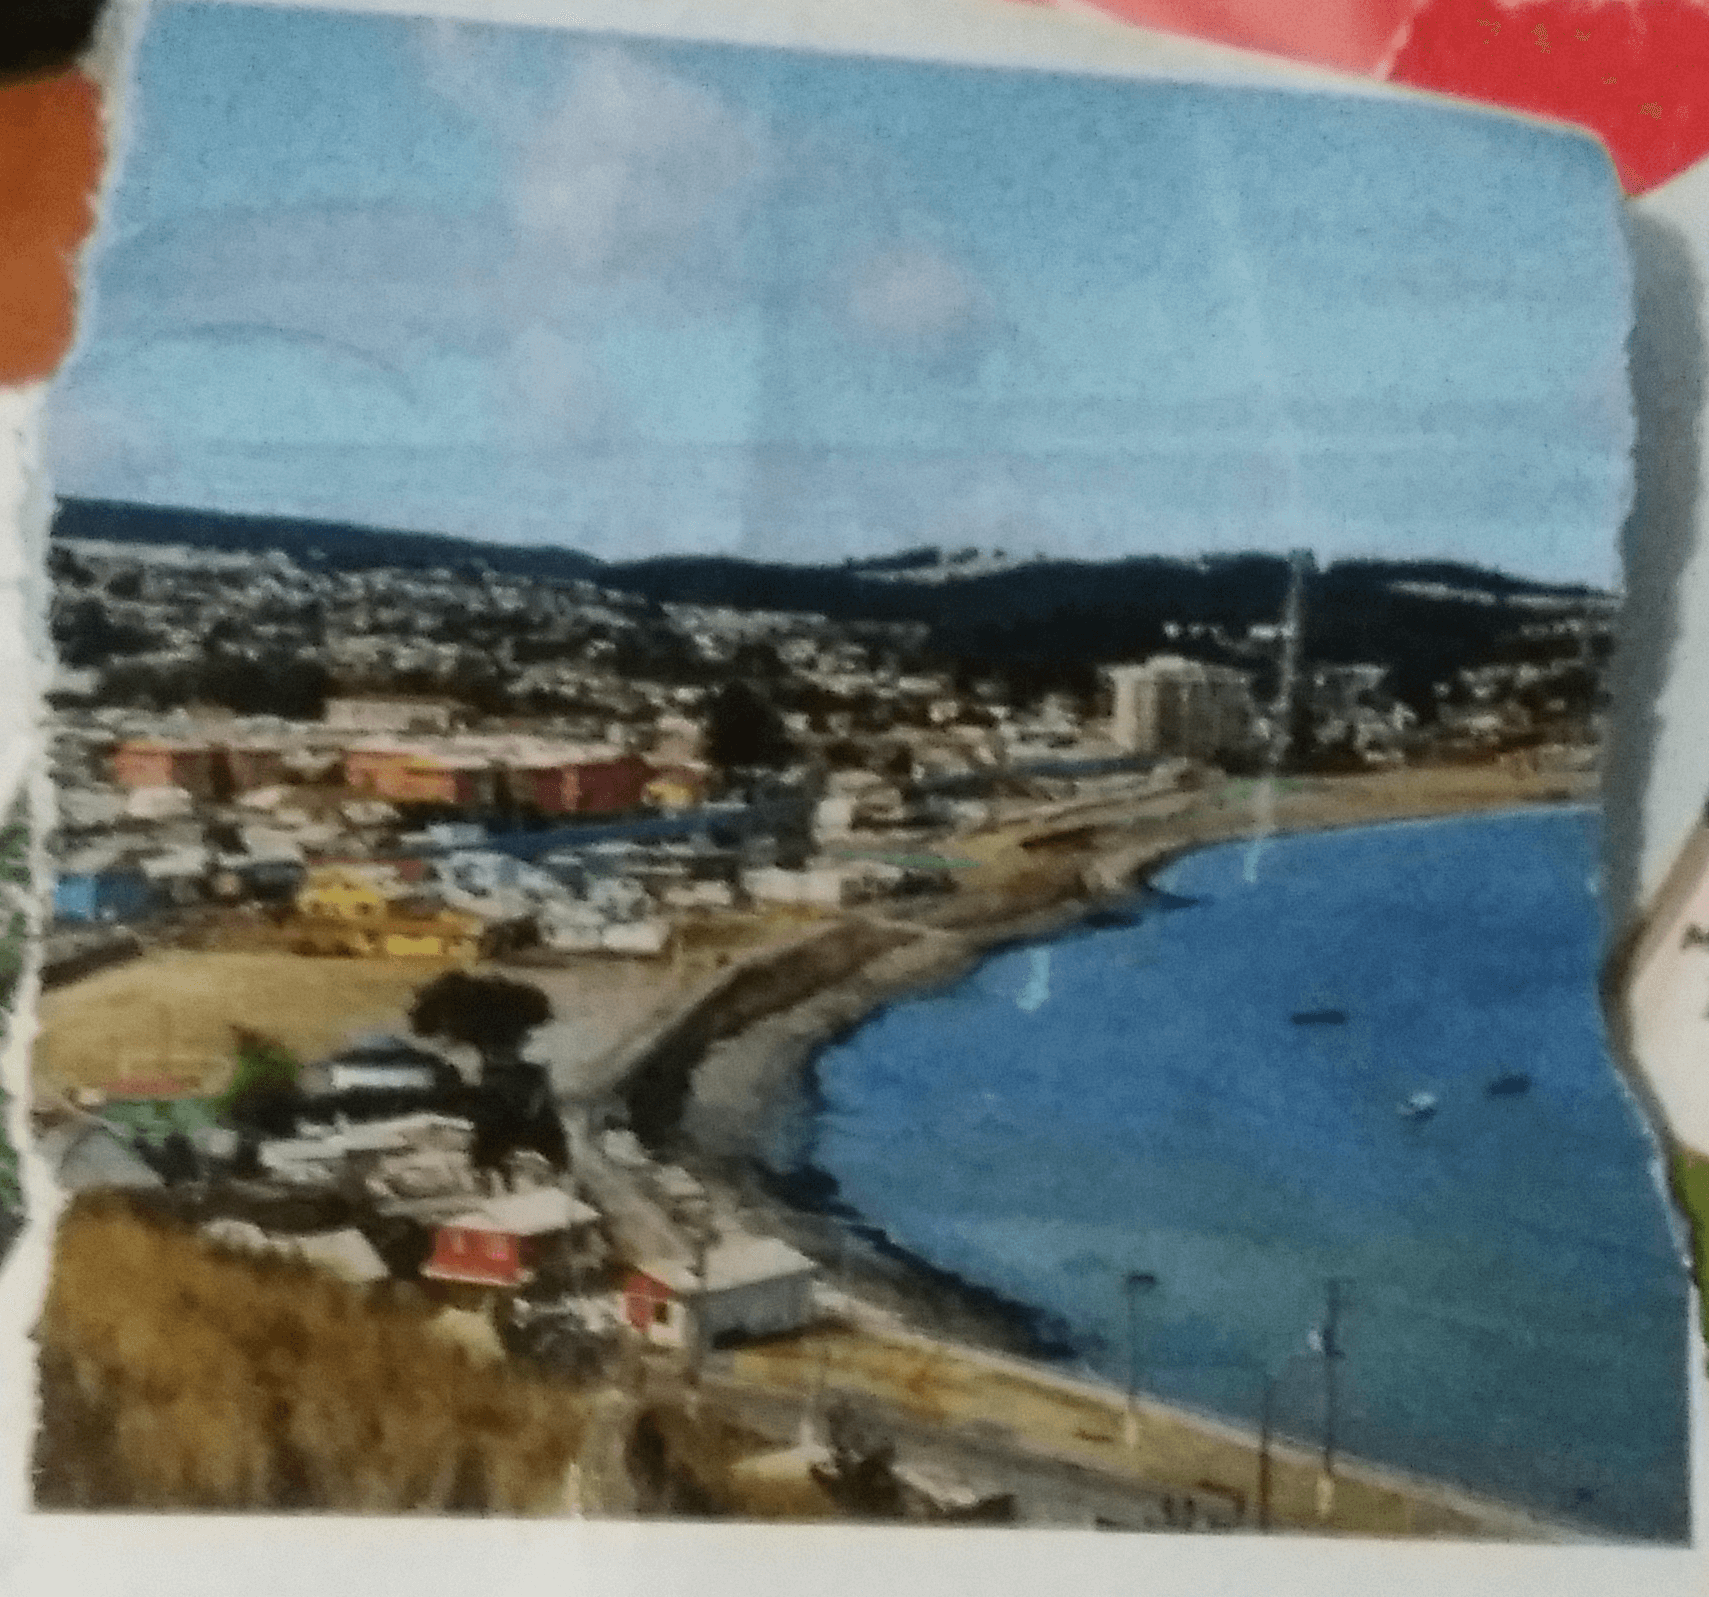
\includegraphics[width=20mm,height=20mm]{marcel1.png} & ``Una casa en la playa, ideal para pasear con la familia'' & ``Representa el compartir con la familia con una situación económica estable'' \\
\hline

2 & 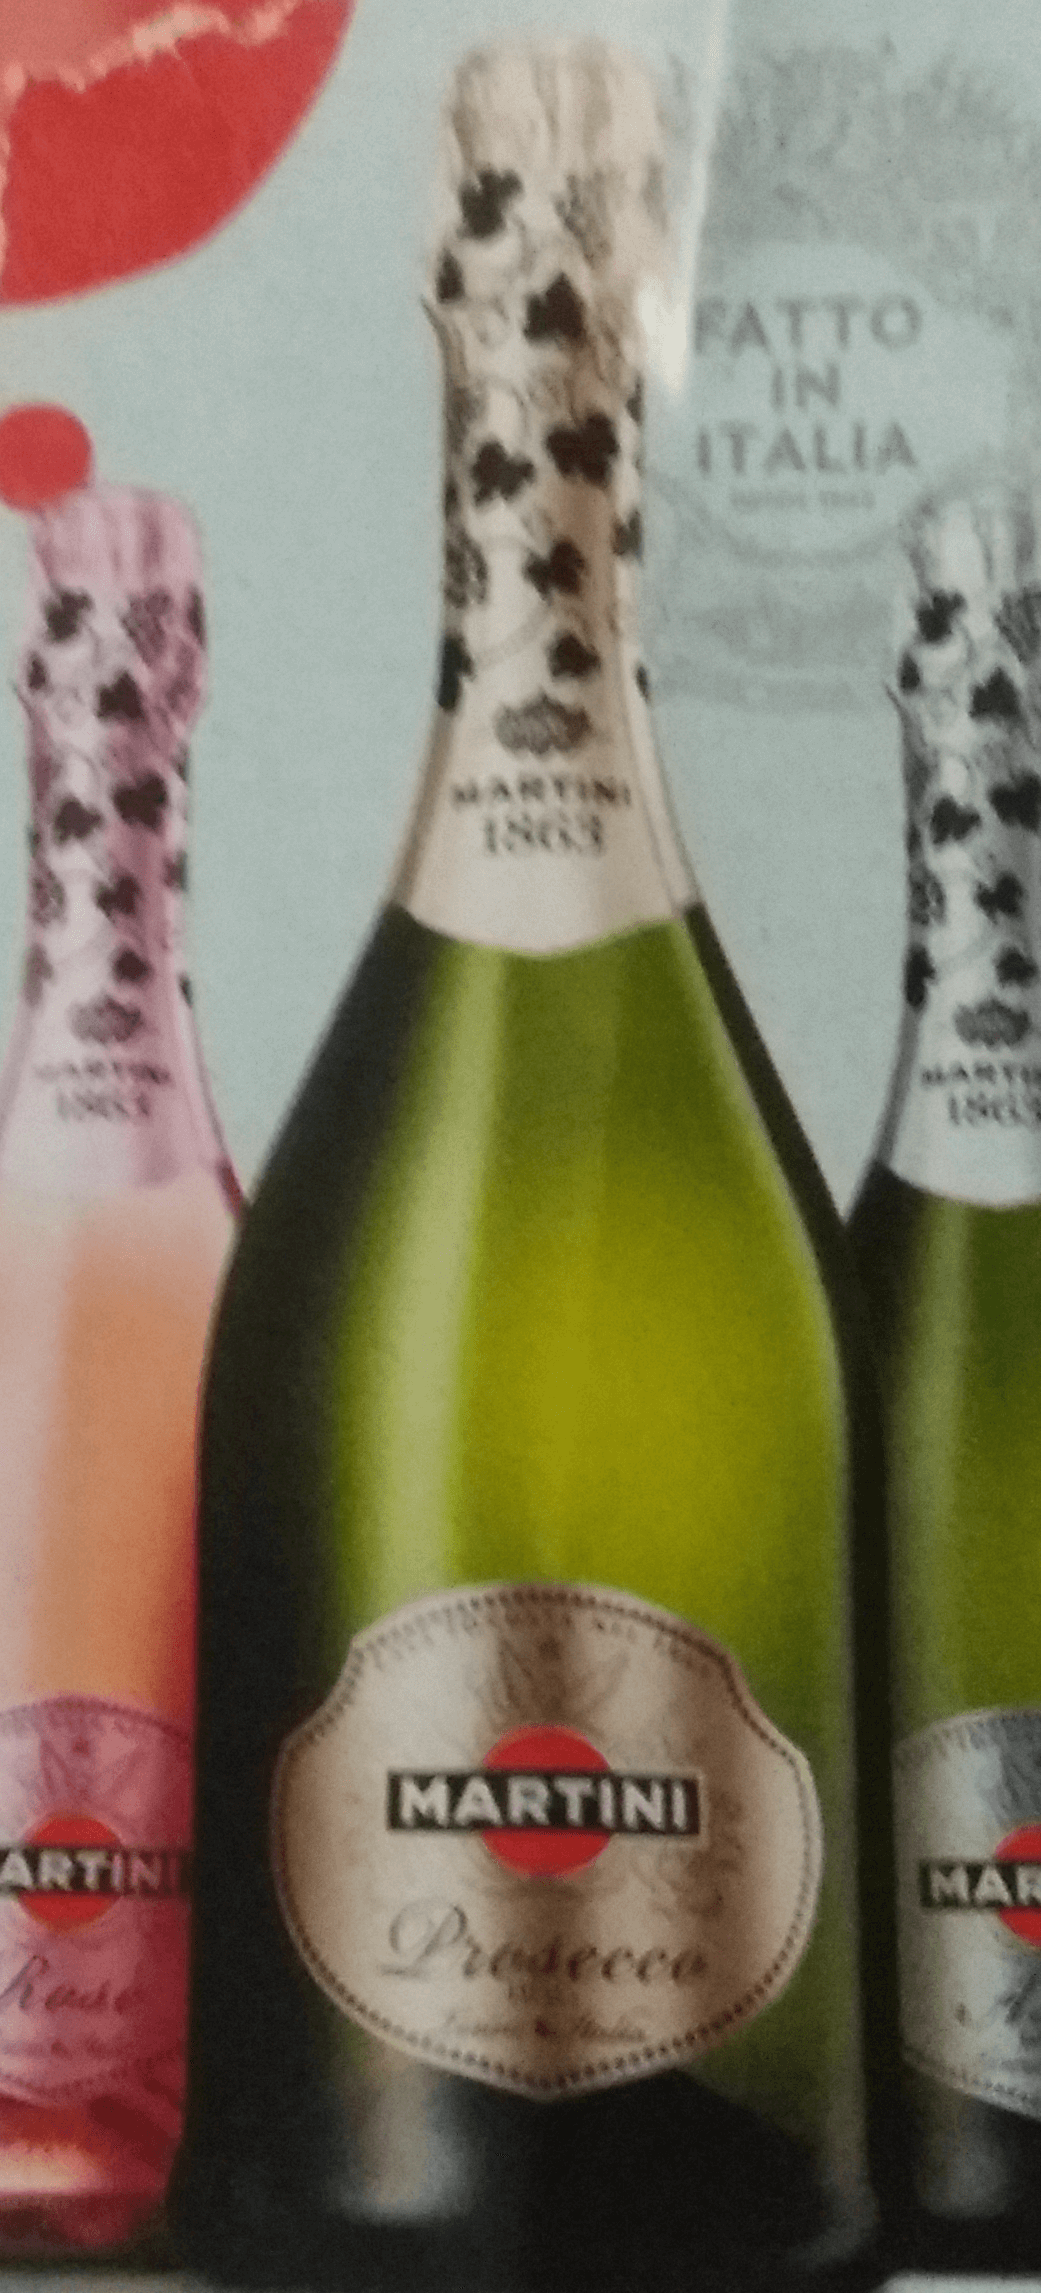
\includegraphics[width=20mm,height=20mm]{marcel2.png} & ``Una botella de champange representa celebración y diversión'' & ``Tener un título, se asocia a disfrutar placeres de la vida'' \\
\hline

3 & 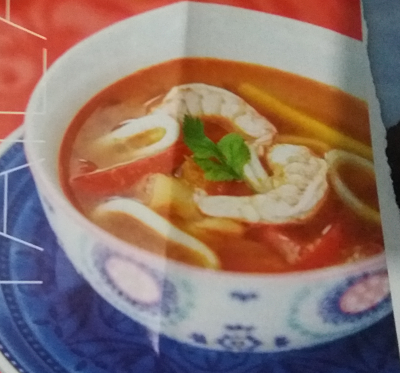
\includegraphics[width=20mm,height=20mm]{marcel3.png} & ``Un plato de comida especial representa los gustos exclusivos que uno se puede dar'' & ``Tener una buena situación económica'' \\
\hline

4 & 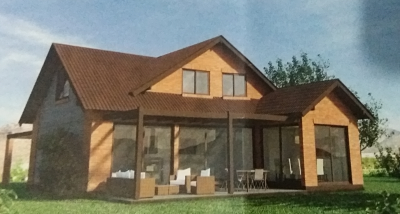
\includegraphics[width=20mm,height=20mm]{marcel5.png} & ``Tener una casa grande para la familia''  & ``El terminar una carrera implica tener un buen trabajo y mucho dinero, con el cual se puede optar a mejores condiciones de vida'' \\
\hline

5 & 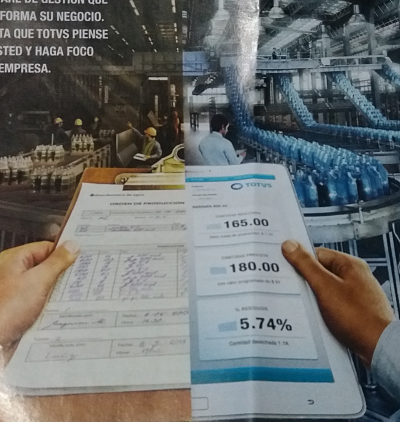
\includegraphics[width=20mm,height=20mm]{marcel6.png} & ``Participación activa en la industria'' & ``Generar aportes al trabajo, ser un buen profesional'' \\
\hline

6 & 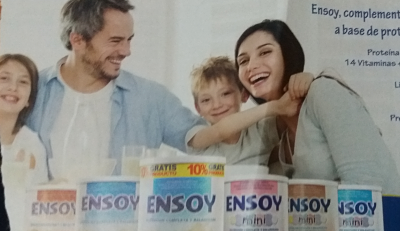
\includegraphics[width=20mm,height=20mm]{marcel7.png} & ``Tener una buena familia'' & ``Generar estabilidad y buenos lazos'' \\
\hline

7 & 
\includegraphics[width=20mm,height=20mm]{marcel8.png} & ``Dar la mano'' &  ``Generar buenos lazos profesionales y hacer negocios'' \\
\hline


\caption{Entrevista 1.}
\label{tabla:marcel}
\end{longtable}

Los grupos de imágenes que escogió el entrevistado fueron:\\

Grupo 1: imágenes 2 y 3, mencionando que son los placeres y gustos que se puede dar uno en la vida.\\

Grupo 2: imágenes 1, 4 y 6, mencionando el lado familiar, de tener algo consolidado y estable.\\

Grupo 3: imágenes 5 y 7, mencionando lado profesional, de tener estabilidad.\\

¿Cómo se ven afectadas tus motivaciones si desertas?.\\
``Los grupos 1 y 3 se complicarían ya que no se podrían lograr sin un título, en cambio el grupo 2 siempre estará porque es la familia''\\* 


\underline {ENTREVISTA 2} \\
Nombre: Fabián\\
Edad: 23\\
Carrera: 4to Año Ingeniería Civil Informática y Telecomunicaciones\\
Comuna: Puente Alto \\

\begin{longtable}{>{\centering\arraybackslash}m{1cm} >{\centering\arraybackslash}m{2cm} >{\arraybackslash}m{5cm}>{\arraybackslash}m{5cm}}
	
	\hline
	Número & Imagen & Descripción & Asociaciones \\
	\hline \hline
	\endfirsthead
	
	\hline
	Número & Imagen & Descripción & Asociaciones \\
	\hline \hline
	\endhead

1 & 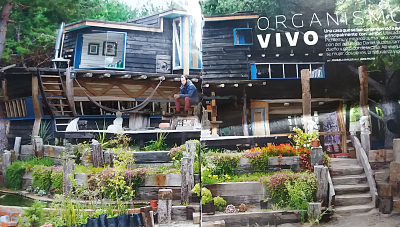
\includegraphics[width=20mm,height=20mm]{fabian1.png} & ``Casa grande'' &  ``Casa acogedora y armónica tanto para él como para su familia''\\
\hline

2 & 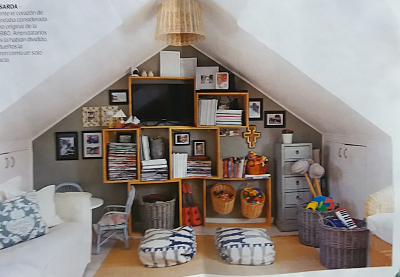
\includegraphics[width=20mm,height=20mm]{fabian2.png} & ``Diseño de espacio vanguardista y acogedor'' & ``Tener un espacio personal grande y vanguardista'' \\
\hline

3 & 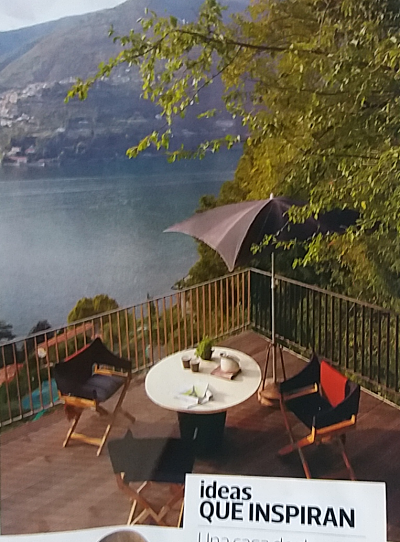
\includegraphics[width=20mm,height=20mm]{fabian3.png} & ``Casa en el lago'' & ``Espacio compartido, acogedor''\\
\hline

4 & 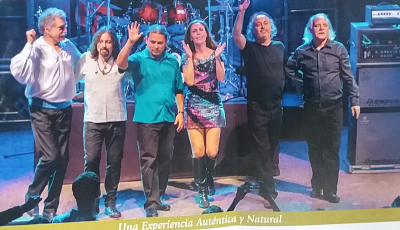
\includegraphics[width=20mm,height=20mm]{fabian4.png} & ``Cultura y música'' &  ``Tener una buena situación económica para disfrutar eventos culturales'' \\
\hline

5 & 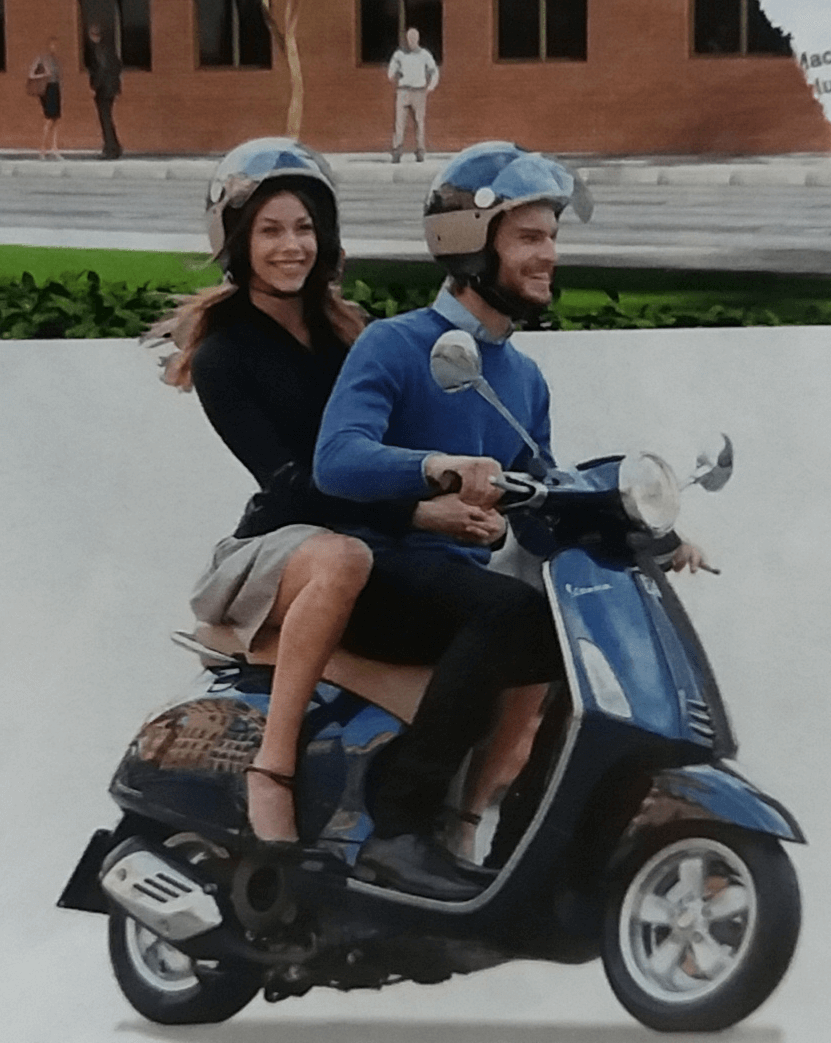
\includegraphics[width=20mm,height=20mm]{fabian5.png} & ``Pareja feliz'' & ``Compañera de vida bajo la premisa de familia, poder ofrecer un buen vivir a través de ser un profesional'' \\
\hline

6 & 
\includegraphics[width=20mm,height=20mm]{fabian6.png} & ``Redes profesionales'' & ``Generar proyectos de ingeniería''\\
\hline

7 & 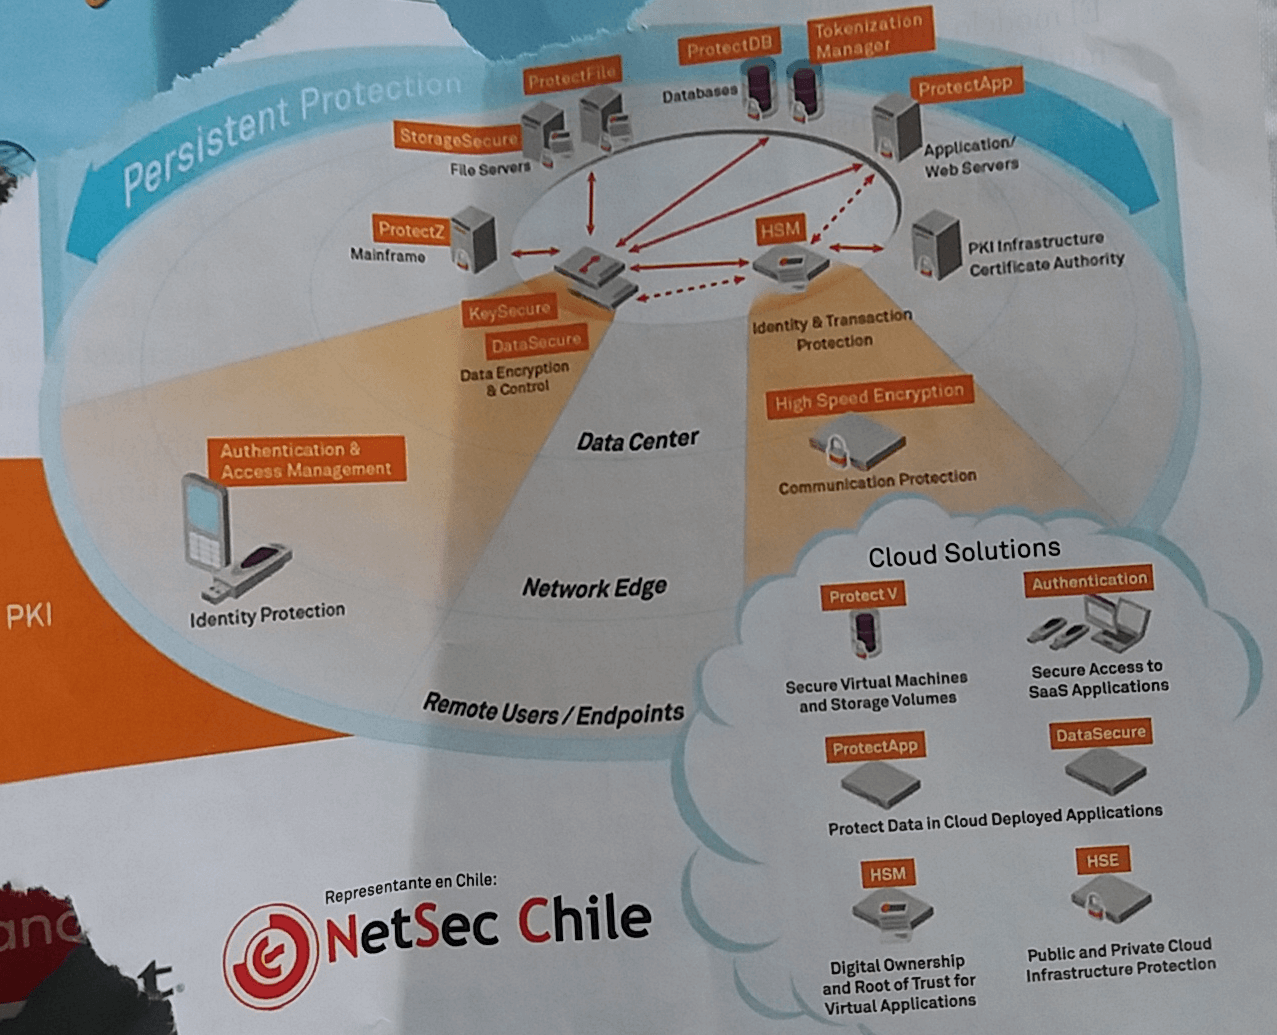
\includegraphics[width=20mm,height=20mm]{fabian7.png} & ``Redes informáticas''  & ``Tener un trabajo relacionado a redes informáticas y ser un buen profesional, para viajar por el mundo'' \\
\hline

8 & 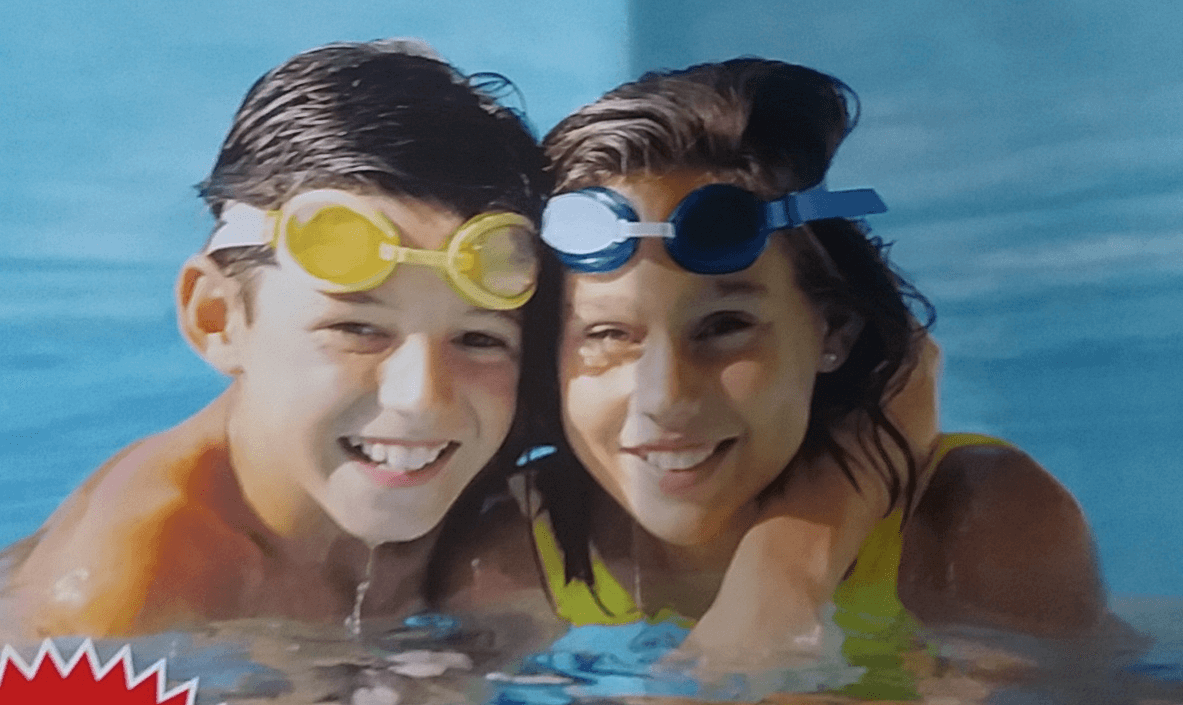
\includegraphics[width=20mm,height=20mm]{fabian8.png} & ``Niños felices'' & ``Sueños de ser papá, de tener las herramientas para dar un buen pasar'' \\
\hline


\caption{Entrevista 2.}
\label{tabla:fabian}
\end{longtable}



Los grupos de imágenes que escogió el entrevistado fueron:\\

Grupo 1: imágenes 4, 6 y 7, mencionando los gustos personales, ligando la parte profesional y la consecuencia de tener el dinero para darse los gustos.\\

Grupo 2: imágenes 5 y 8, mencionando la parte familiar.\\

Grupo 3: imágenes 1, 2, 3  mencionando la parte del hogar, una parte de acogida y en donde compartir.\\

¿Cómo se ven afectadas tus motivaciones si desertas?.\\

``Generaría mucha frustración, ya que la carrera es una herramienta para poder tener todo lo de las imágenes''\\


\underline {ENTREVISTA 3} \\* 
Nombre: Cristian\\
Edad: 25\\
Carrera: 5to Año Ingeniería Civil Informática y Telecomunicaciones\\
Comuna: La Florida\\

\begin{longtable}{>{\centering\arraybackslash}m{1cm} >{\centering\arraybackslash}m{2cm} >{\arraybackslash}m{5cm}>{\arraybackslash}m{5cm}}
	
	\hline
	Número & Imagen & Descripción & Asociaciones \\
	\hline \hline
	\endfirsthead
	
	\hline
	Número & Imagen & Descripción & Asociaciones \\
	\hline \hline
	\endhead

1 & 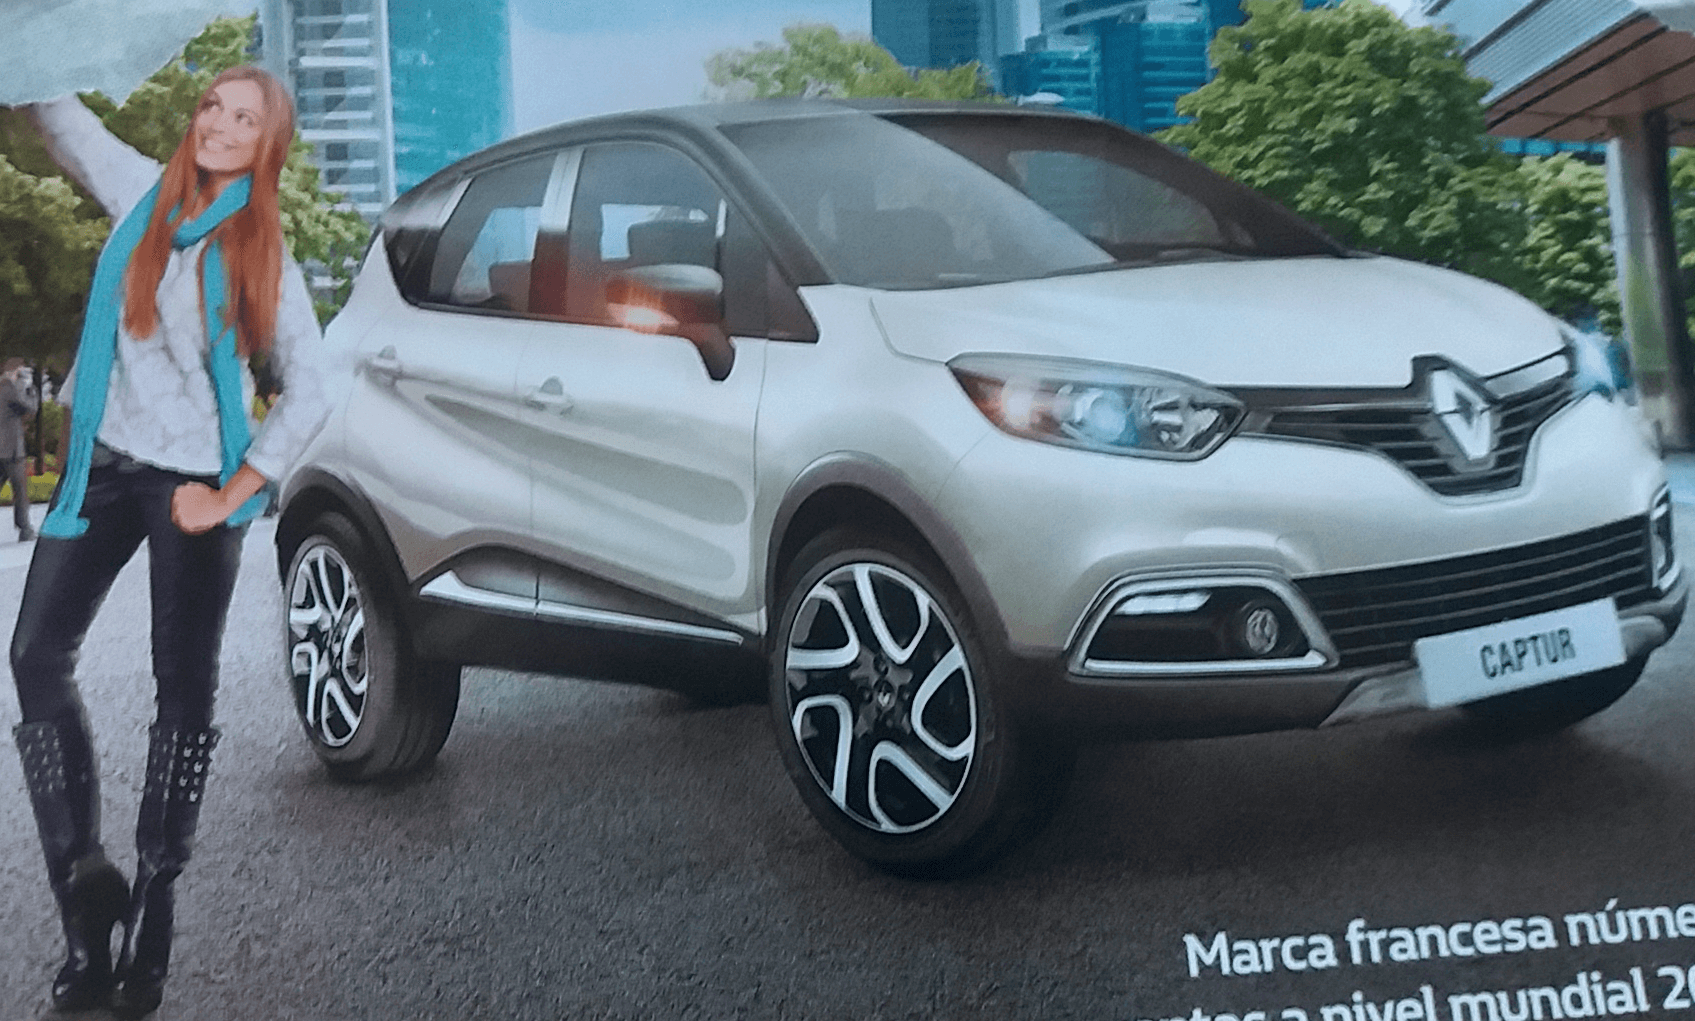
\includegraphics[width=20mm,height=20mm]{cristian1.png} & ``Auto'' & ``Tener un auto para tener independencia'' \\
\hline

2 & 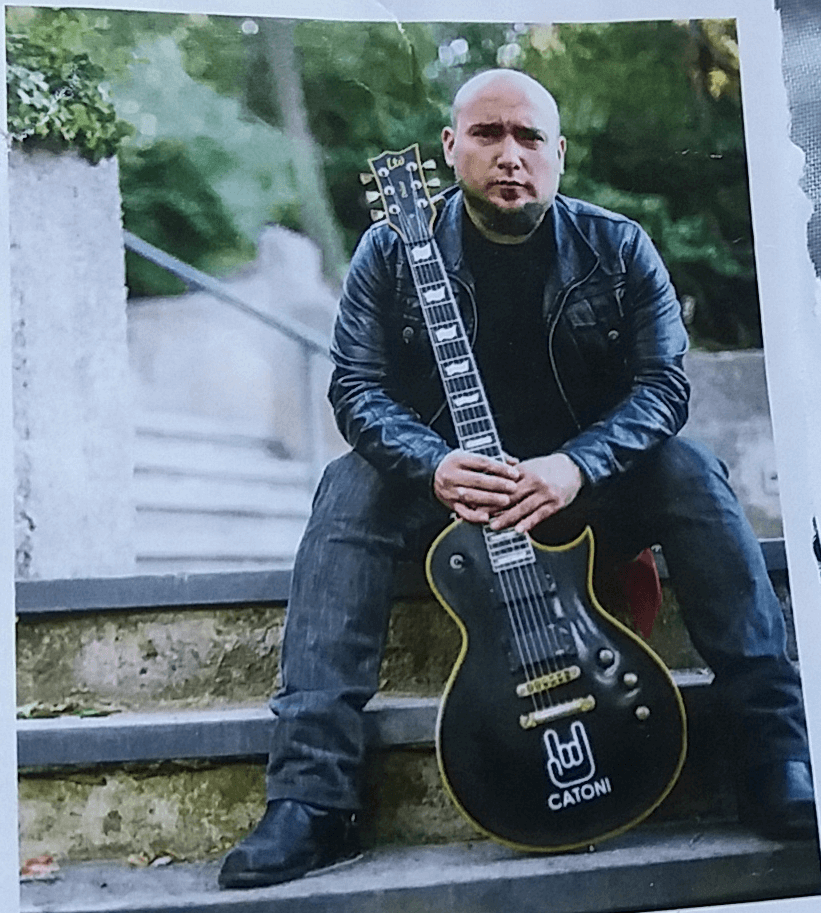
\includegraphics[width=20mm,height=20mm]{cristian2.png} & ``Guitarra'' & ``Tener sus gustos, la música'' \\
\hline

3 & 
\includegraphics[width=20mm,height=20mm]{cristian3.png} & ``Seguridad informática'' & ``Poder dedicarse a la seguridad informática'' \\
\hline

4 & 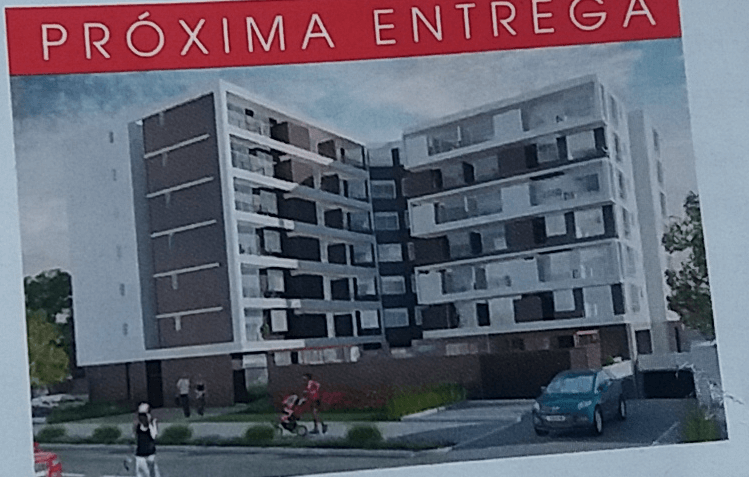
\includegraphics[width=20mm,height=20mm]{cristian4.png} & ``Departamentos'' & ``Tener un lugar donde vivir'' \\
\hline

5 & 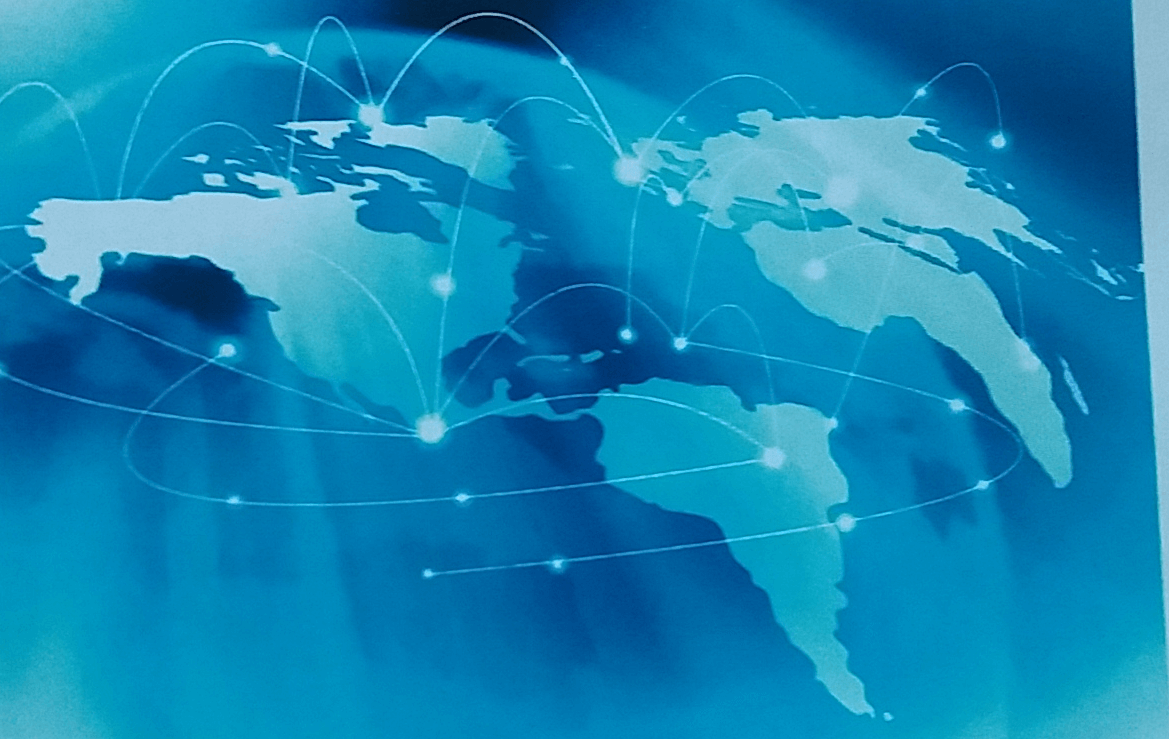
\includegraphics[width=20mm,height=20mm]{cristian5.png} & ``Mundo'' & ``Poder realizar viajes por el mundo''\\
\hline

6 & 
\includegraphics[width=20mm,height=20mm]{cristian6.png} & ``Cerveza'' & ``Poder darse sus gustos''\\
\hline

7 & 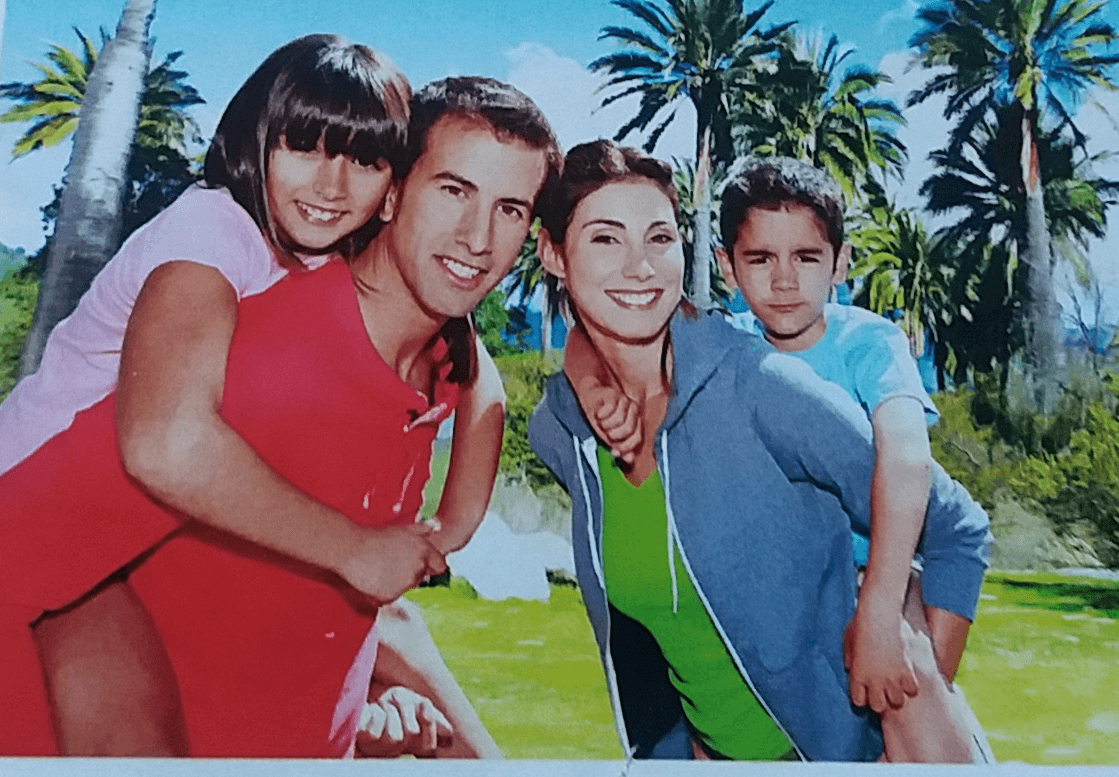
\includegraphics[width=20mm,height=20mm]{cristian7.png} & ``La familia'' & ``Tener una familia y tener plata para mantener a la familia'' \\
\hline

8 & 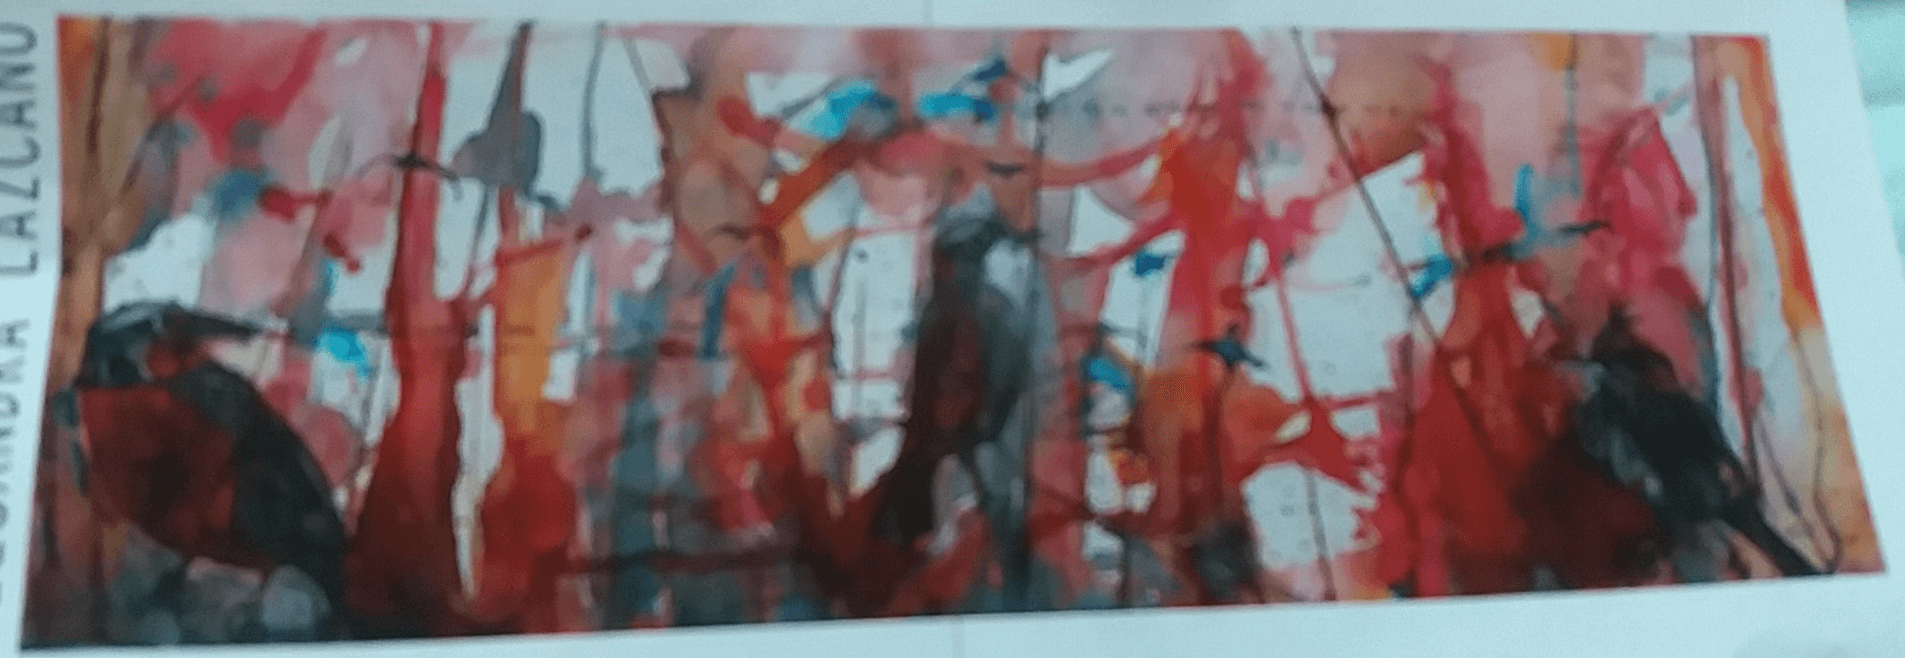
\includegraphics[width=20mm,height=20mm]{cristian8.png} & ``Decoración'' & ``Tener su casa decorada''\\
\hline


\caption{Entrevista 3.}
\label{tabla:cristian}
\end{longtable}

Los grupos de imágenes que escogió el entrevistado fueron:\\

Grupo 1: imágenes 1, 2 y 5, mencionando gustos personales, viajar a diferentes partes del mundo \\

Grupo 2: imágenes 3, 4 y 7, mencionando la parte familiar, trabajando en lo que le gusta, teniendo su casa y familia.\\

Grupo 3: imágenes 6 y 8, mencionando que son gustos exclusivos, no tan importantes como los del grupo 1.\\

¿Cómo se ven afectadas tus motivaciones si desertas?.\\

``Solamente podría tener la parte familiar, los otros grupos serían bastante complicados de satisfacer''\\


\underline {ENTREVISTA 4} \\*
Nombre: Manuel\\
Edad: 24\\
Carrera: 4to Año Ingeniería Civil Informática y Telecomunicaciones\\
Comuna: Providencia\\

\begin{longtable}{>{\centering\arraybackslash}m{1cm} >{\centering\arraybackslash}m{2cm} >{\arraybackslash}m{5cm}>{\arraybackslash}m{5cm}}
	
	\hline
	Número & Imagen & Descripción & Asociaciones \\
	\hline \hline
	\endfirsthead
	
	\hline
	Número & Imagen & Descripción & Asociaciones \\
	\hline \hline
	\endhead

1 & 
\includegraphics[width=20mm,height=20mm]{manuel1.png} & ``Linux'' & ``Tener sus trabajos realizados en Linux''\\
\hline

2 & 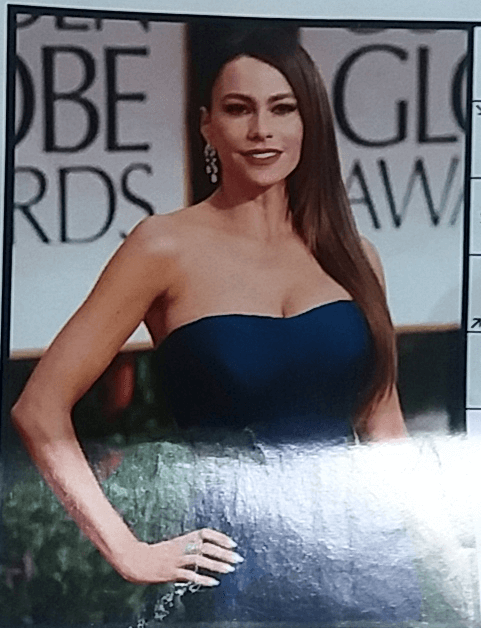
\includegraphics[width=20mm,height=20mm]{manuel2.png} & ``Mujer'' & ``Tener una linda mujer''\\
\hline

3 & 
\includegraphics[width=20mm,height=20mm]{manuel3.png} & ``Pan'' & ``Tener para comer y una vida sana'' \\
\hline

4 & 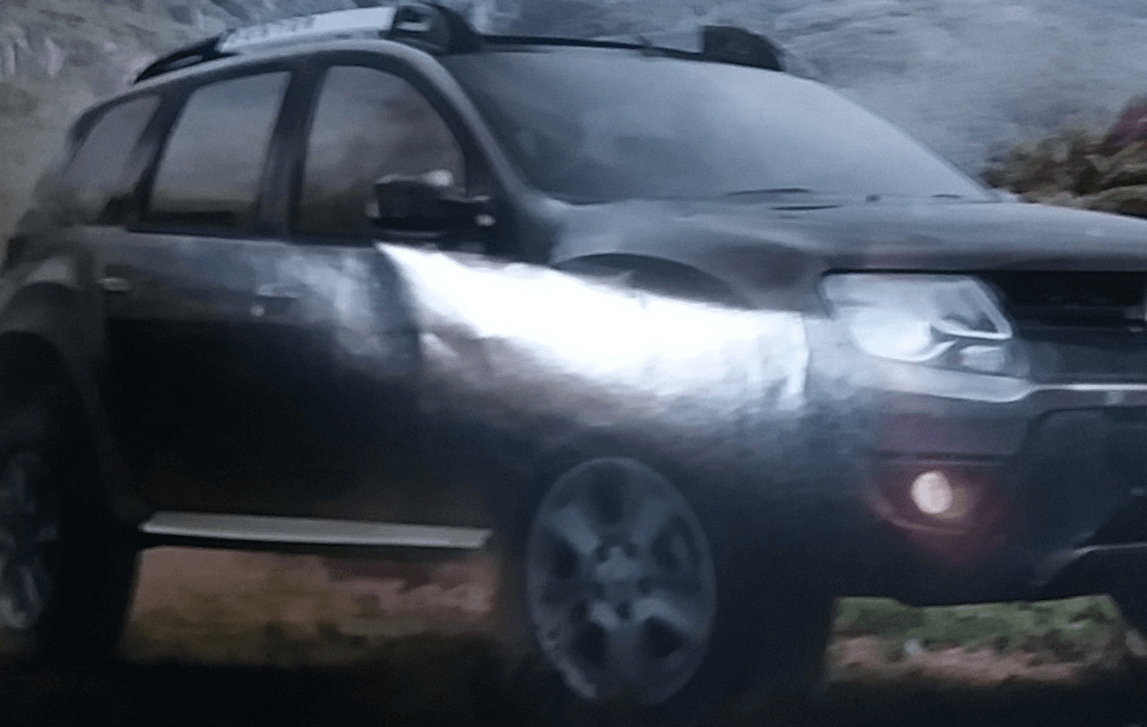
\includegraphics[width=20mm,height=20mm]{manuel4.png} & ``Auto'' & ``Tener suficiente trabajo para comprar un auto familiar'' \\
\hline

5 & 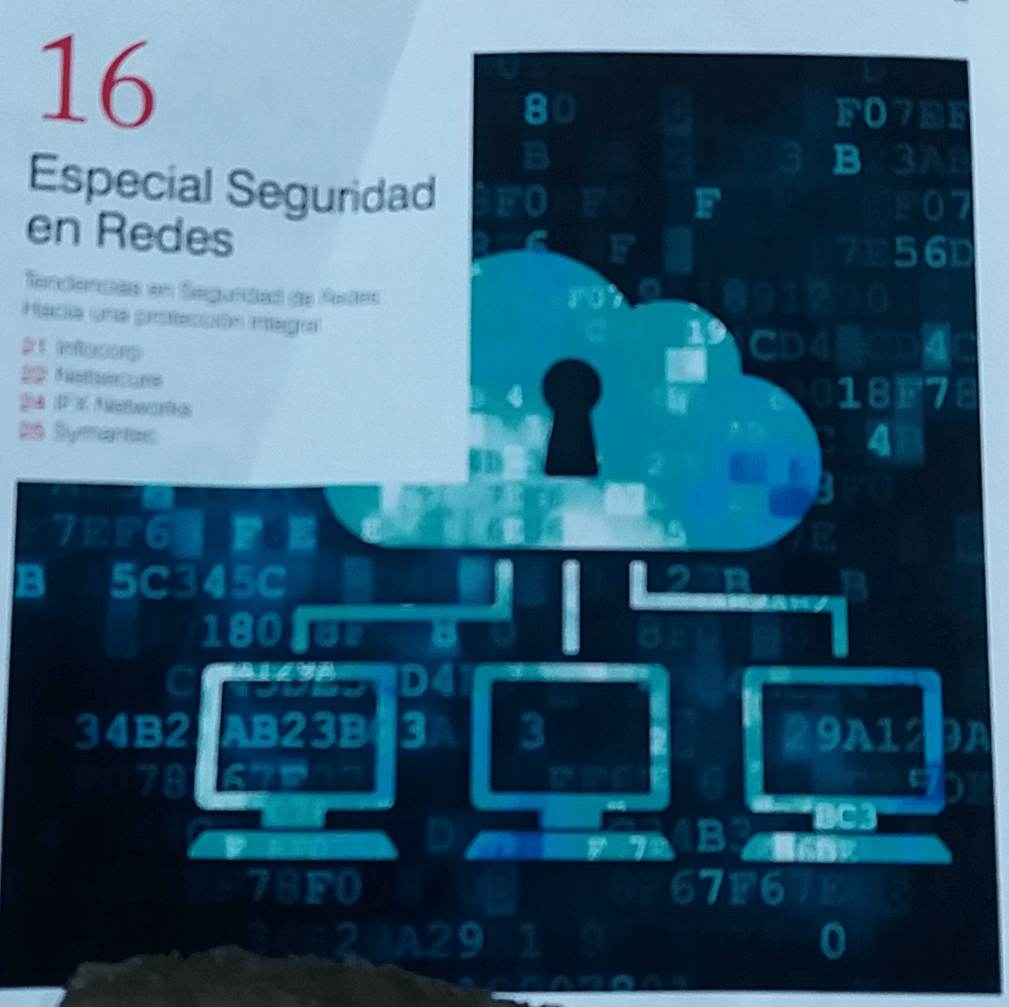
\includegraphics[width=20mm,height=20mm]{manuel5.png} & ``Redes informáticas'' & ``Tener un trabajo en el área de redes informáticas'' \\
\hline

6 & 
\includegraphics[width=20mm,height=20mm]{manuel6.png} & ``Seguridad informática'' & ``Poder desempeñarse en el área de seguridad informática'' \\
\hline

7 & 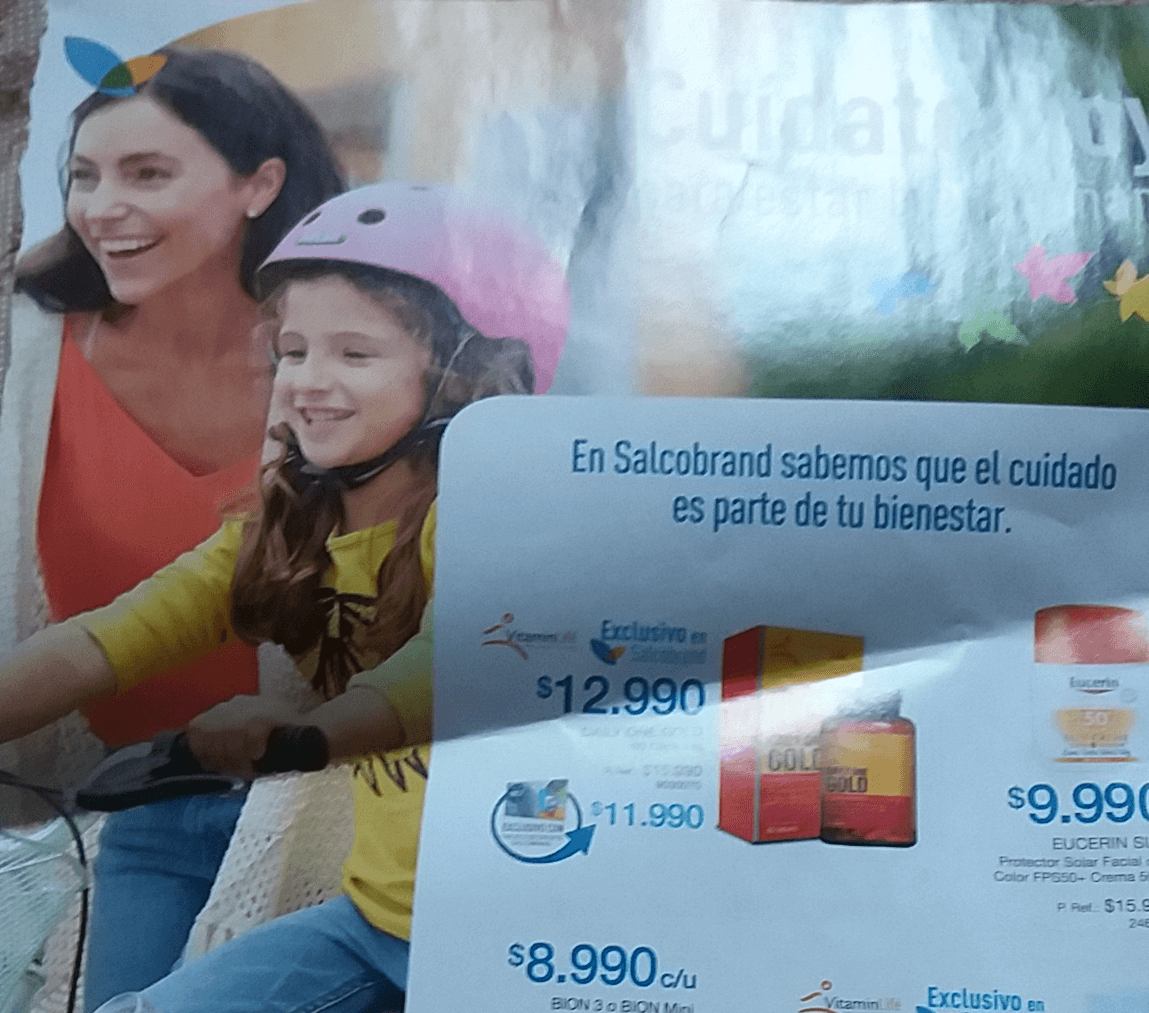
\includegraphics[width=20mm]{manuel7.png} & ``Madre e hija'' & ``Tener una familia con una hija sana'' \\
\hline


\caption{Entrevista 4.}
\label{tabla:manuel}
\end{longtable}

Los grupos de imágenes que escogió el entrevistado fueron:\\

Grupo 1: imágenes 2, 3, 4 y 7, mencionando que es la vida familiar. \\

Grupo 2: imágenes 1, 5 y 6 mencionando que es la vida trabajo.\\


¿Cómo se ven afectadas tus motivaciones si desertas?.\\

``No habría suficiente dinero para sustentar todo''\\

\underline {ENTREVISTA 5} \\*
Nombre: Cristian\\
Edad: 23\\
Carrera: 4to Año Psicología\\
Comuna: Antofagasta\\

\begin{longtable}{>{\centering\arraybackslash}m{1cm} >{\centering\arraybackslash}m{2cm} >{\arraybackslash}m{5cm}>{\arraybackslash}m{5cm}}
	
	\hline
	Número & Imagen & Descripción & Asociaciones \\
	\hline \hline
	\endfirsthead
	
	\hline
	Número & Imagen & Descripción & Asociaciones \\
	\hline \hline
	\endhead

1 & 
\includegraphics[width=20mm,height=20mm]{cristiant1.jpg} & ``Inexperto'' & ``Falta de experiencia al terminar la carrera, motiva a trabajar'' \\
\hline

2 & 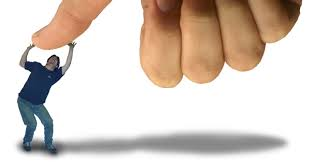
\includegraphics[width=20mm,height=20mm]{cristiant2.jpg} & ``Presión'' & ``Cerrar una etapa de la vida, para pasar a una siguiente'' \\
\hline

3 & 
\includegraphics[width=20mm,height=20mm]{cristiant3.jpg} & ``Profesional'' & ``Estar listo para enfrentar el mundo laboral'' \\
\hline

4 & 
\includegraphics[width=20mm,height=20mm]{cristiant4.jpg} & ``Biblioteca'' & ``Dejar atrás los libros'' \\
\hline

5 & 
\includegraphics[width=20mm,height=20mm]{cristiant5.jpg} & ``Superación'' & ``Sentir la sensación de éxito''  \\
\hline

6 & 
\includegraphics[width=20mm,height=20mm]{cristiant6.jpg} & ``Deudas'' & ``Tener mayores responsabilidades''\\
\hline

7 & 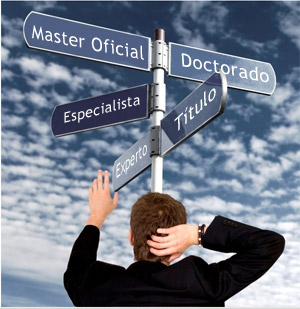
\includegraphics[width=20mm,height=20mm]{cristiant7.jpg} & ``Magister'' & ``Poder sacar un postgrado'' \\
\hline


\caption{Entrevista 5.}
\label{tabla:cristiant}
\end{longtable}

Los grupos de imágenes que escogió el entrevistado fueron:\\

Grupo 1: imágenes 3, 4 y 5, mencionando que representa el éxito y el sentirse realizado por completar la carrera \\

Grupo 2: imágenes 1, 2, 6 y 7, mencionando la incertidumbre de enfrentar el mundo laboral.\\


¿Cómo se ven afectadas tus motivaciones si desertas?.\\

``Afectaría en la complicación de tener que pagar el crédito con aval del estado''\\


\underline {ENTREVISTA 6}\\*
Nombre: Gabriel\\
Edad: 24\\
Carrera: 5to Año Psicología\\
Comuna: Santiago Centro\\

\begin{longtable}{>{\centering\arraybackslash}m{1cm} >{\centering\arraybackslash}m{2cm} >{\arraybackslash}m{5cm}>{\arraybackslash}m{5cm}}
	
	\hline
	Número & Imagen & Descripción & Asociaciones \\
	\hline \hline
	\endfirsthead
	
	\hline
	Número & Imagen & Descripción & Asociaciones \\
	\hline \hline
	\endhead

1 & 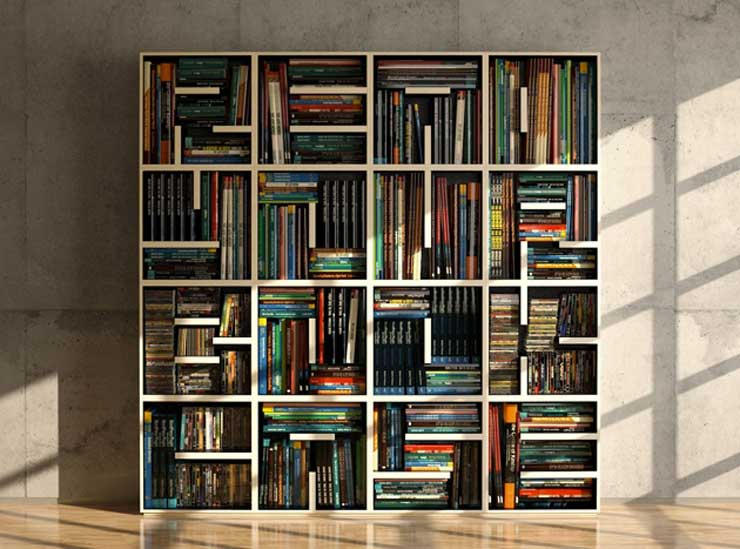
\includegraphics[width=20mm,height=20mm]{gabriel1.jpg} & ``Librero'' & ``Tener muchos libros por el gusto de leer'' \\
\hline

2 & 
\includegraphics[width=20mm,height=20mm]{gabriel2.jpg} & ``Psicología clínica'' & ``Dedicarse a su profesión'' \\
\hline

3 & 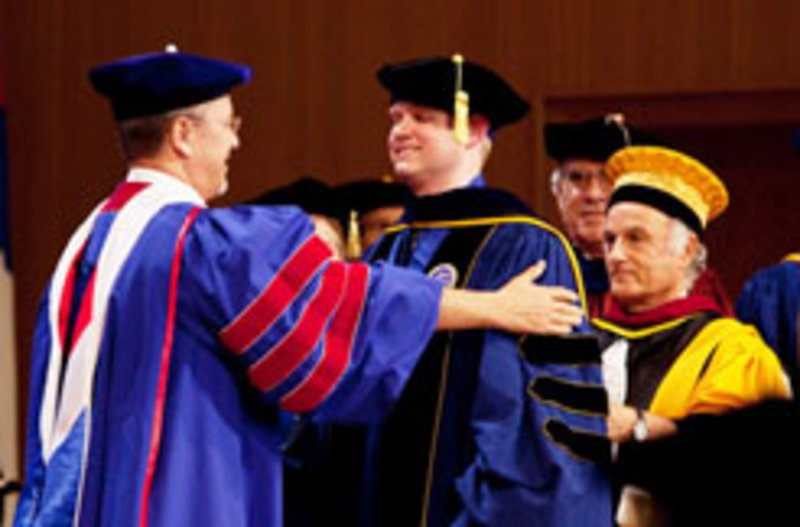
\includegraphics[width=20mm,height=20mm]{gabriel3.jpg} & ``Graduado'' & ``Significa el cierre y el comienzo de una nueva etapa''`` \\
\hline

4 & 
\includegraphics[width=20mm,height=20mm]{gabriel4.jpg} & ``Autonomía'' & ``Ser una persona independiente'' \\
\hline

5 & 
\includegraphics[width=20mm,height=20mm]{gabriel5.jpg} & ``Deudas'' & ``Al titularse se tendrán muchas deudas'' \\
\hline

6 & 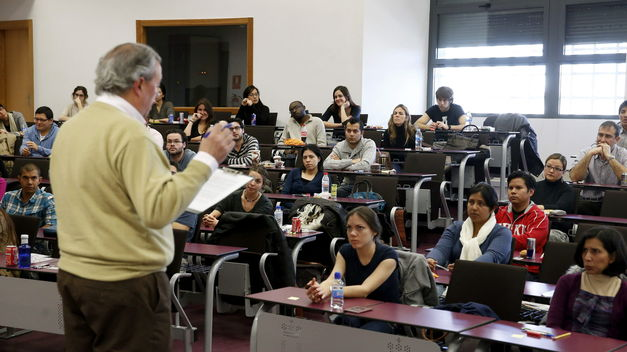
\includegraphics[width=20mm,height=20mm]{gabriel6.jpg} & ``Profesor'' & ``Poder dar clases en un futuro''\\
\hline


\caption{Entrevista 6.}
\label{tabla:gabriel}
\end{longtable}

Los grupos de imágenes que escogió el entrevistado fueron:\\

Grupo 1: imágenes 1, 2, 3 y 6, mencionando que representa la independencia \\

Grupo 2: imágenes 4 y 5, mencionando que refleja el capitalismo y que siempre habrán deudas.\\


¿Cómo se ven afectadas tus motivaciones si desertas?.\\

``Afectaría en la complicación de tener independencia''\\


\underline {ENTREVISTA 7}\\*
Nombre: Tania \\
Edad: 24\\
Carrera: 4to Año Ingeniería Civil Industrial \\
Comuna: Peñalolen \\

\begin{longtable}{>{\centering\arraybackslash}m{1cm} >{\centering\arraybackslash}m{2cm} >{\arraybackslash}m{5cm}>{\arraybackslash}m{5cm}}
	
	\hline
	Número & Imagen & Descripción & Asociaciones \\
	\hline \hline
	\endfirsthead
	
	\hline
	Número & Imagen & Descripción & Asociaciones \\
	\hline \hline
	\endhead

1 & 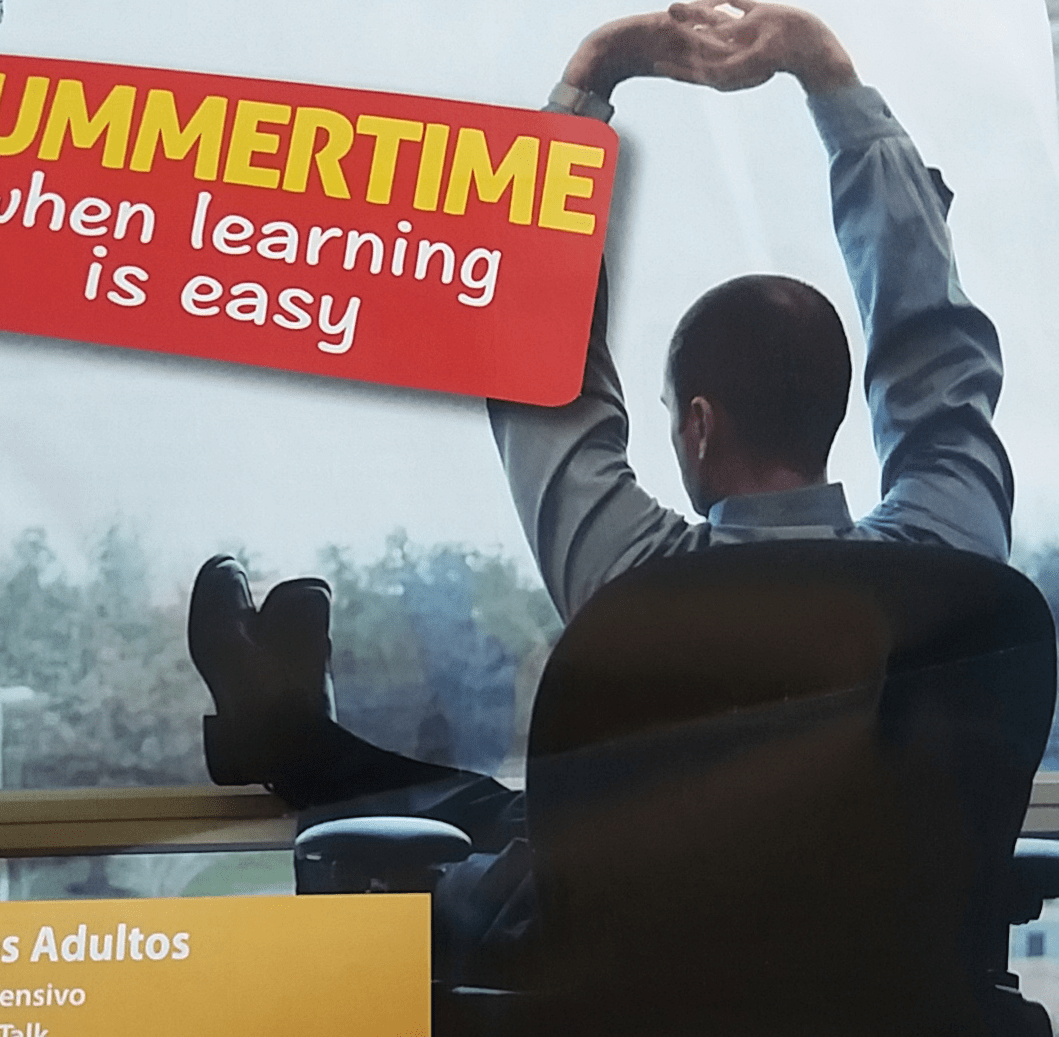
\includegraphics[width=20mm,height=20mm]{tania1.png} & ``Libertad laboral'' & ``Trabajar de forma independiente'' \\
\hline

2 & 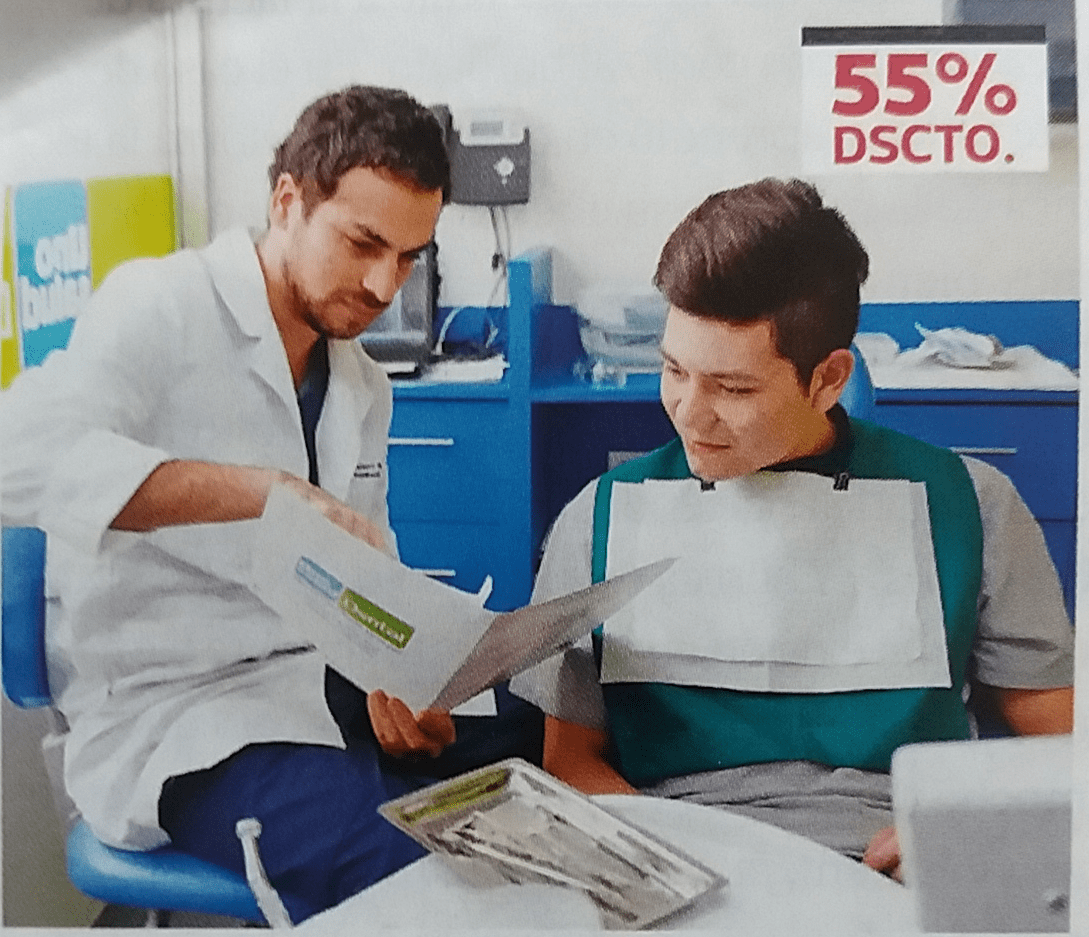
\includegraphics[width=20mm,height=20mm]{tania2.png} & ``Salud'' & ``Poder tener el dinero para obtener buenos tratamientos médicos'' \\
\hline

3 & 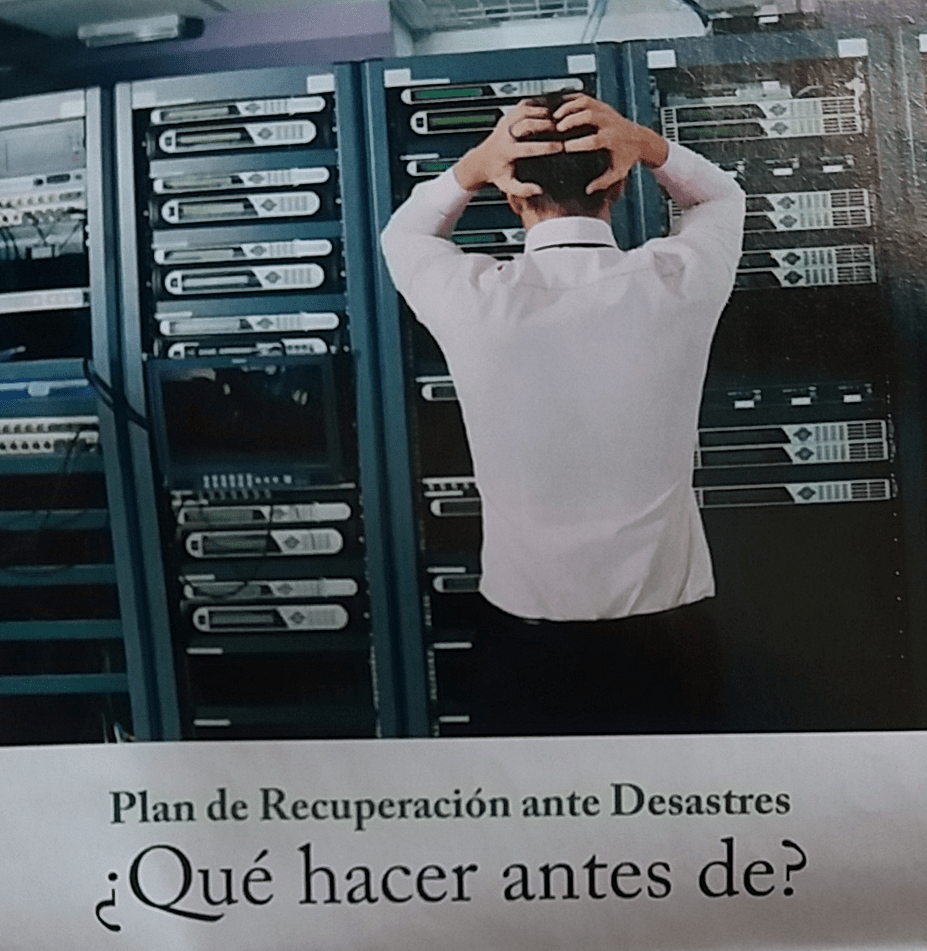
\includegraphics[width=20mm,height=20mm]{tania3.png} & ``¿Qué hacer?'' & ``Necesidad de dinero y experiencia'' \\
\hline

4 & 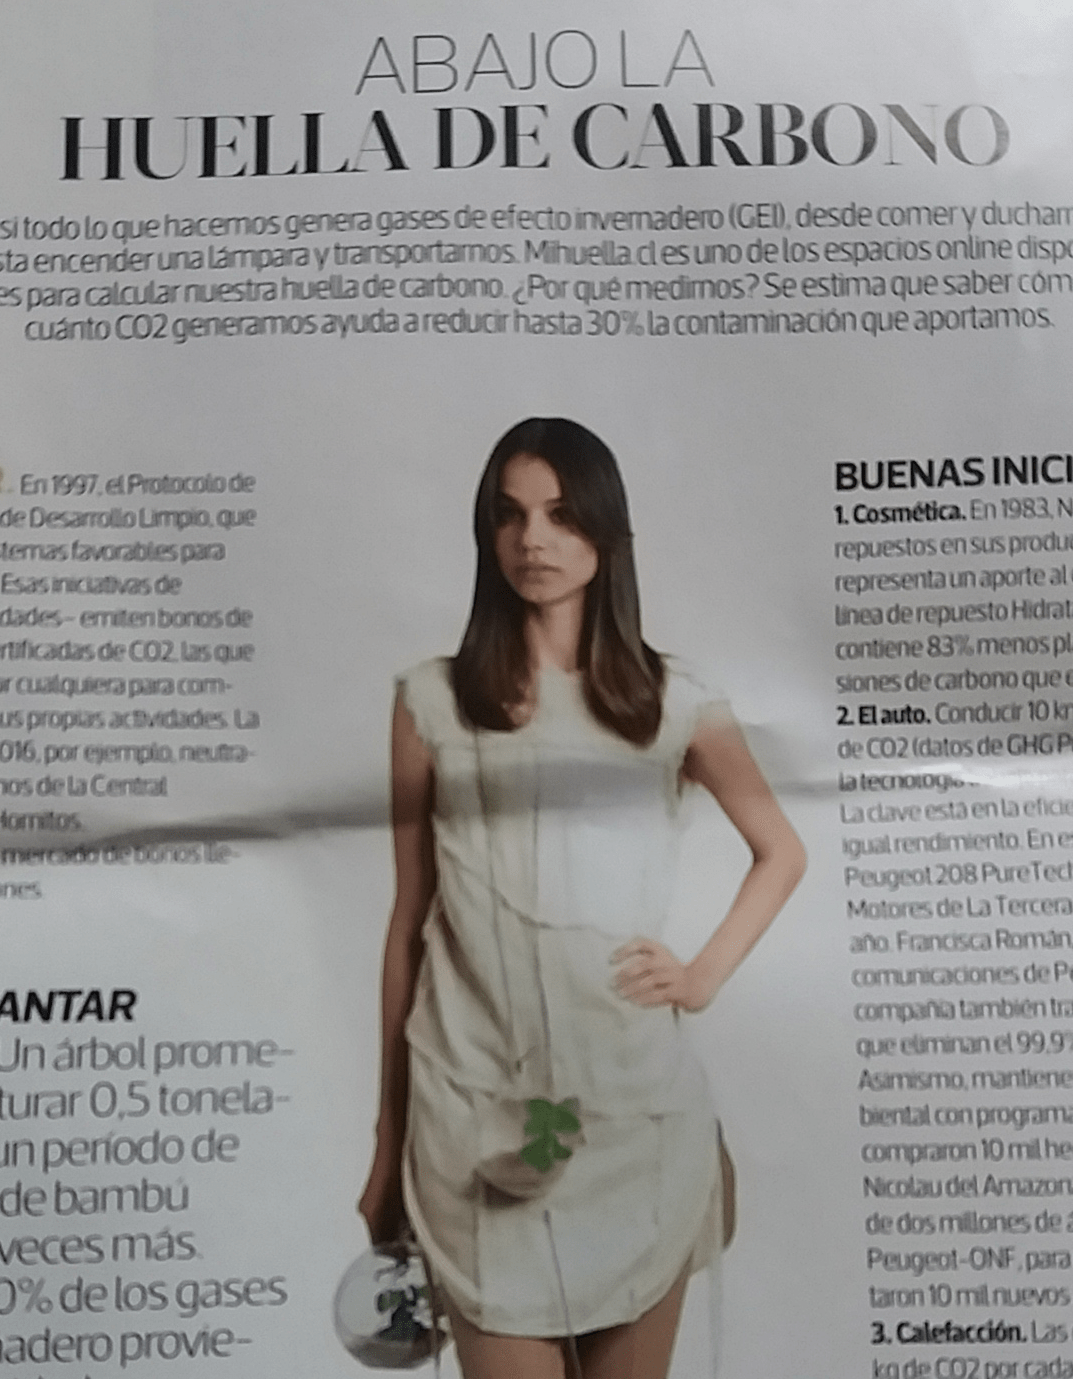
\includegraphics[width=20mm,height=20mm]{tania4.png} & ``Estilo de vida'' & ``Vida consciente con el planeta, a largo plazo'' \\
\hline

5 & 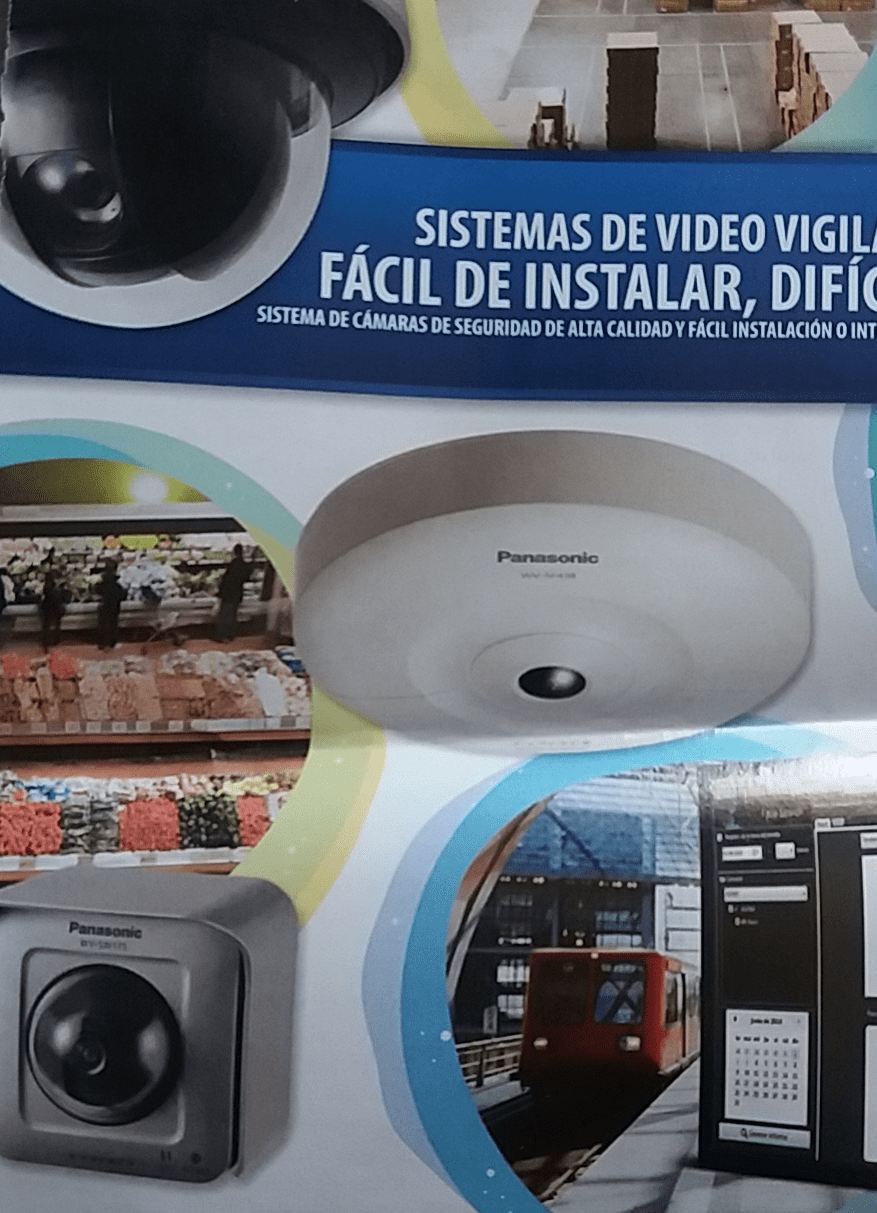
\includegraphics[width=20mm,height=20mm]{tania5.png} & ``Seguridad'' & ``Desarrollar seguridad personal'' \\
\hline

6 & 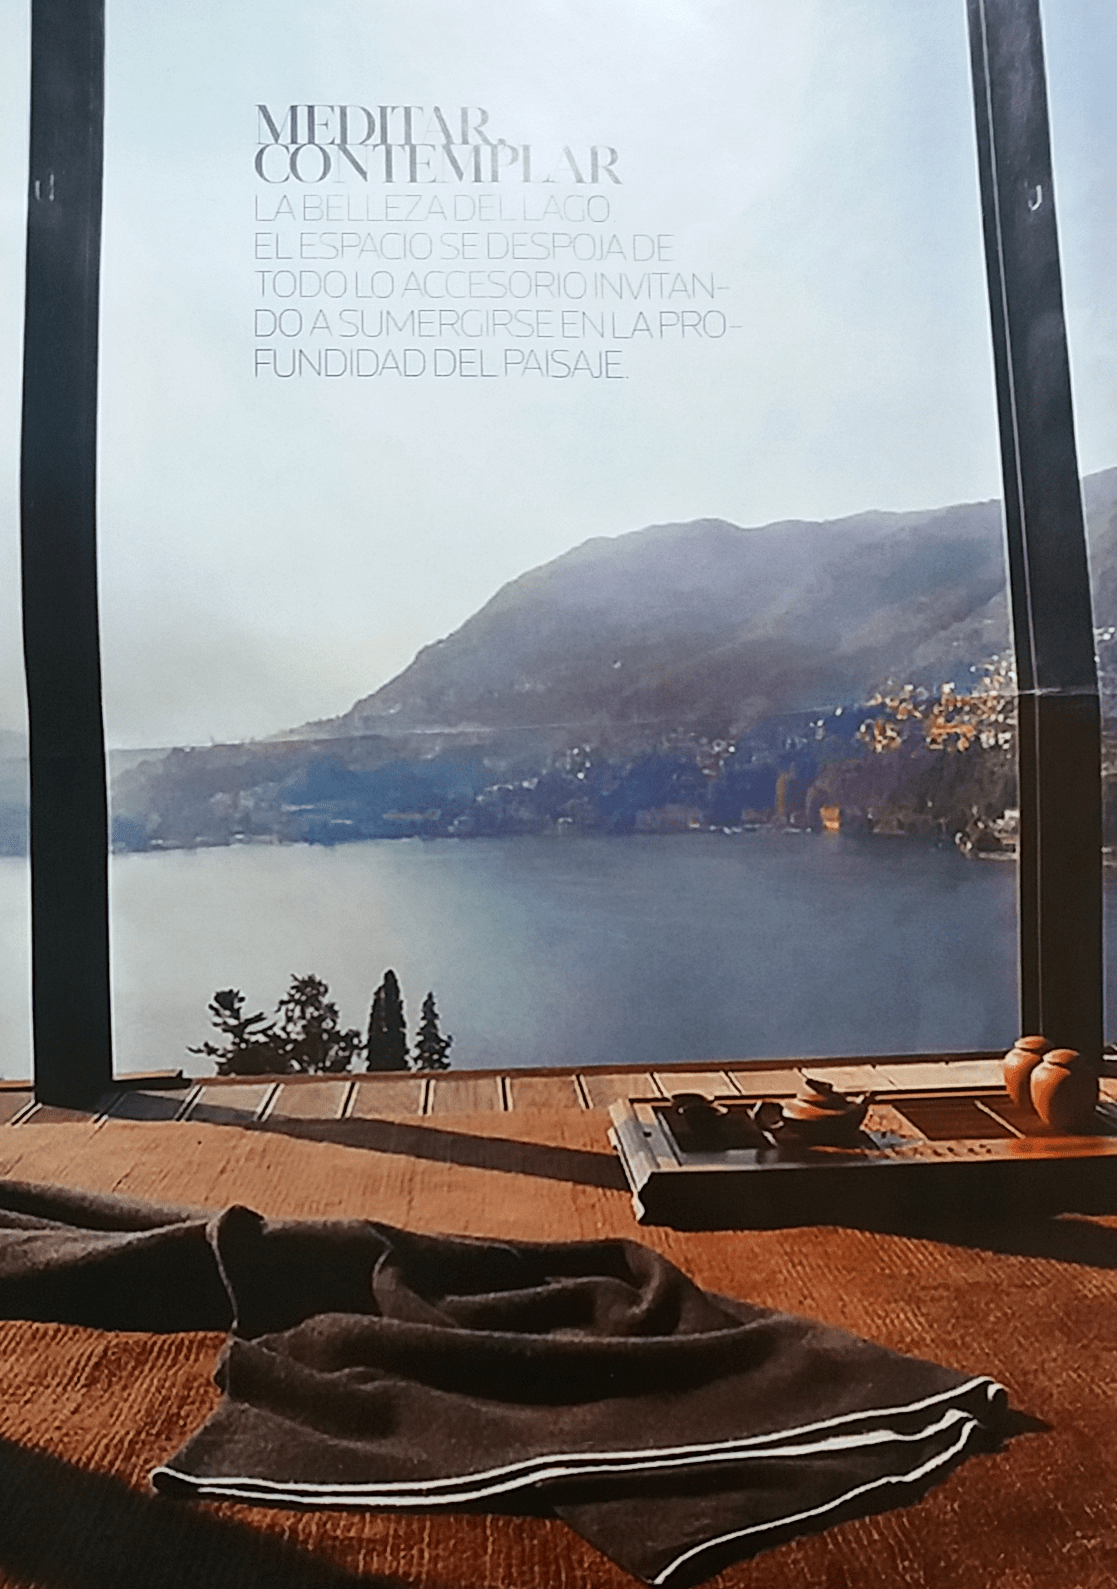
\includegraphics[width=20mm,height=20mm]{tania6.png} & ``Viajes'' & ``Tener la disponibilidad de tiempo y dinero, salir de la rutina, tener una vida más relajada''\\
\hline

7 & 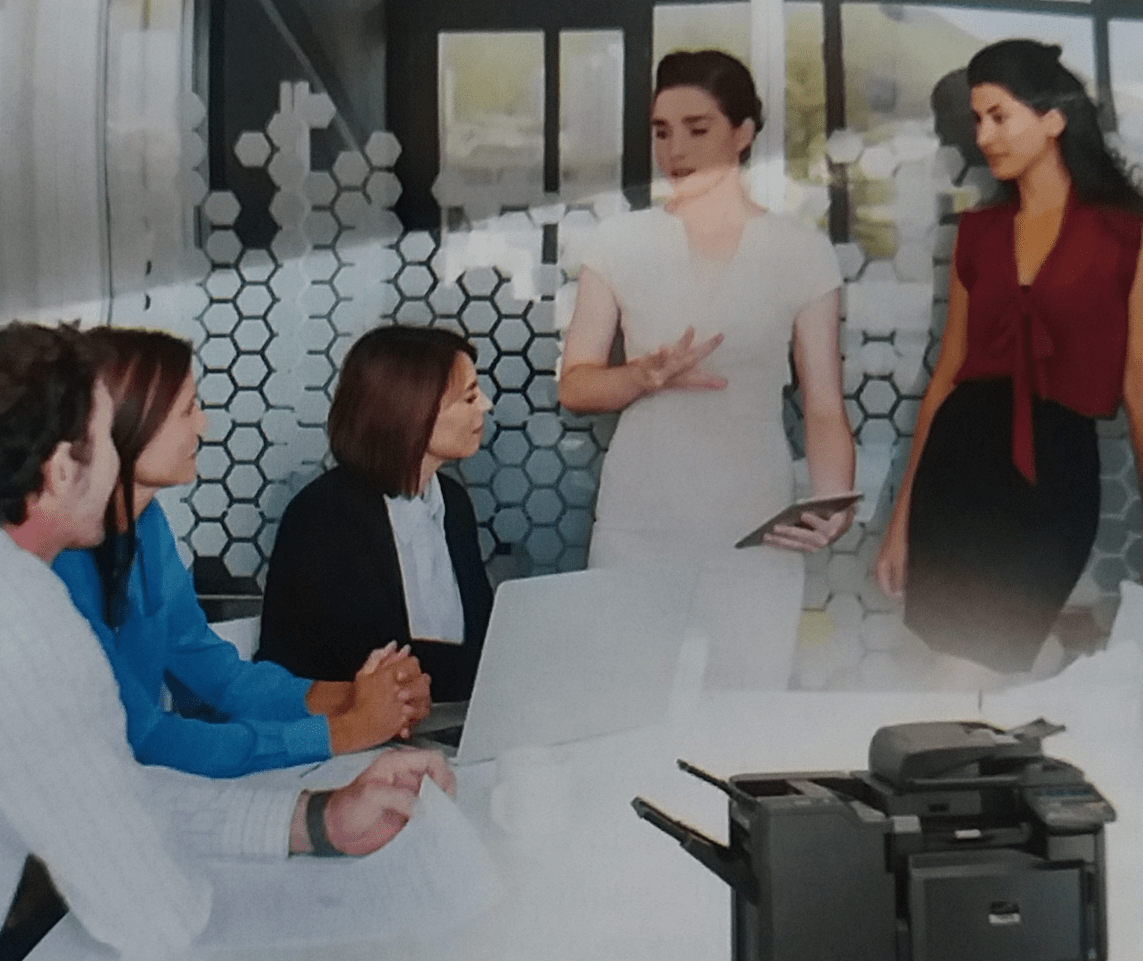
\includegraphics[width=20mm,height=20mm]{tania7.png} & ``Trabajo estable'' & ``Trabajar con personas, tener vida social''\\
\hline

\caption{Entrevista 7.}
\label{tabla:tania}
\end{longtable}

Los grupos de imágenes que escogió el entrevistado fueron:\\

Grupo 1: imágenes 1, 4 y 6, mencionando que representa tranquilidad y bienestar espiritual, relacionando el trabajo independiente que da libertad, complementándose con su estilo de vida y viajes.  \\

Grupo 2: imágenes 2 y 5, mencionando que representa seguridad, tener seguridad con su salud y frente a la delincuencia.\\

Grupo 3: imágenes 3 y 7, mencionando que representa el ámbito laboral, el no saber en que trabajará, pero si tener una idea de que trabajará con un grupo de gente y hacer vida social.\\

¿Cómo se ven afectadas tus motivaciones si desertas?.\\

``Solo se verían cumplidas las imágenes del grupo 1 y muy a largo plazo, los otros grupos no los podría cumplir''


\underline {ENTREVISTA 8}\\*
Nombre: Carlos\\
Edad: 22 \\
Carrera: 3er Año Ingeniería Comercial\\
Comuna: Santiago Centro\\

\begin{longtable}{>{\centering\arraybackslash}m{1cm} >{\centering\arraybackslash}m{2cm} >{\arraybackslash}m{5cm}>{\arraybackslash}m{5cm}}
	
	\hline
	Número & Imagen & Descripción & Asociaciones \\
	\hline \hline
	\endfirsthead
	
	\hline
	Número & Imagen & Descripción & Asociaciones \\
	\hline \hline
	\endhead

1 & \includegraphics[width=20mm,height=20mm]{carlos1.png} & ``Tranquilidad'' & ``Terminar una carrera transmite seguridad y sentirse útil para algo'' \\
\hline

2 & \includegraphics[width=20mm,height=20mm]{carlos2.png} & ``Presentación de Apple'' & ``Representa el triunfo que puede llegar a tener como profesional.'' \\
\hline

3 & \includegraphics[width=20mm,height=20mm]{carlos3.png} & ``Triunfo''' & ``Reconocimiento por llegar a una meta'' \\
\hline

4 & \includegraphics[width=20mm,height=20mm]{carlos4.png} & ``Tiempo libre'' & ``Expresa los pasatiempos que se pueden realizar al terminar la carrera'' \\
\hline

5 & \includegraphics[width=20mm,height=20mm]{carlos5.png} & ``Pasatiempos'' & ``Poder tener la libertad de darse tiempos libres y hacer las cosas que uno quiere'' \\
\hline

6 & \includegraphics[width=20mm,height=20mm]{carlos6.png} & ``Trabajo'' & ``Trabajar de forma relajada, ya que con el título tienes una base para dedicarse a lo que te gusta'' \\
\hline



\caption{Entrevista 8.}
\label{tabla:carlos}
\end{longtable}

Los grupos de imágenes que escogió el entrevistado fueron:\\


Grupo 1: imágenes 1, 4 y 5, mencionando que representa el tiempo libre, que ya obtenido un título, ya tienes una base para poder tener dinero y dedicarse a gustos más caros. \\

Grupo 2: imágenes 2, 3 y 6, mencionando que representa el triunfo, el éxito de terminar una meta.\\


¿Cómo se ven afectadas tus motivaciones si desertas?.\\

``En lo personal tener un título no es el único camino para cumplir mis sueños, la sociedad impone que debe ser así, pero yo no lo veo como la única opción.''


\underline {ENTREVISTA 9}\\*
Nombre: Ilana\\
Edad: 23\\
Carrera: 3er Año Ingeniería Comercial\\
Comuna: Las Condes \\

\begin{longtable}{>{\centering\arraybackslash}m{1cm} >{\centering\arraybackslash}m{2cm} >{\arraybackslash}m{5cm}>{\arraybackslash}m{5cm}}
	
	\hline
	Número & Imagen & Descripción & Asociaciones \\
	\hline \hline
	\endfirsthead
	
	\hline
	Número & Imagen & Descripción & Asociaciones \\
	\hline \hline
	\endhead

1 & \includegraphics[width=20mm,height=20mm]{ilana1.png} & ``Comida'' & ``Dedicar tiempo para mi persona y realizar lo que me gusta, la cocina.'' \\
\hline

2 & \includegraphics[width=20mm,height=20mm]{ilana2.png} & ``Curso de inglés'' & ``Tener tiempo para poder realizar un curso de inglés y viajar al extranjero.'' \\
\hline

3 & \includegraphics[width=20mm,height=20mm]{ilana3.png} & ``Libertad'' & ``Terminar la carrera, da una sensación de libertad y triunfo.'' \\
\hline

4 & \includegraphics[width=20mm,height=20mm]{ilana4.png} & ``Viajes'' & ``Después de la carrera hay tiempo para disfrutar y conocer el mundo.'' \\
\hline

5 & \includegraphics[width=20mm,height=20mm]{ilana5.png} & ``Independencia'' & ``Poder vivir sola y tener mi departamento.'' \\
\hline

6 & \includegraphics[width=20mm,height=20mm]{ilana6.png} & ``Trabajo'' & ``Encontrar un trabajo en una empresa prestigiosa.'' \\
\hline

\caption{Entrevista 9.}
\label{tabla:ilana}
\end{longtable}

Los grupos de imágenes que escogió el entrevistado fueron:\\

Grupo 1: imágenes 1 y 3, mencionando que representa el relajo y el poder realizar sus gustos, como cocinar. \\

Grupo 2: imágenes 2 y 4, mencionando que representa los viajes, y que aprender un idioma nuevo abre las puertas a conocer otros lugares.\\

Grupo 3: imágenes 5 y 6, mencionado que representa su independencia, para poder tener su departamento, necesita de un trabajo.\\


¿Cómo se ven afectadas tus motivaciones si desertas?.\\

``Seria difícil cumplir el grupo 3, no podría hacer el grupo 2, solamente me podría dedicar a las imágenes del grupo 1.'' \\


\underline {ENTREVISTA 10}\\*
Nombre: Oscar\\
Edad: 28\\
Carrera: 6to Año Ingeniería Civil en Informática y Telecomunicaciones \\
Comuna: Macul \\

\begin{longtable}{>{\centering\arraybackslash}m{1cm} >{\centering\arraybackslash}m{2cm} >{\arraybackslash}m{5cm}>{\arraybackslash}m{5cm}}
	
	\hline
	Número & Imagen & Descripción & Asociaciones \\
	\hline \hline
	\endfirsthead
	
	\hline
	Número & Imagen & Descripción & Asociaciones \\
	\hline \hline
	\endhead

1 & \includegraphics[width=20mm,height=20mm]{oscar1.png} & ``Scooter'' & ``Representa el vehículo que podría adquirir teniendo recursos'' \\
\hline

2 & \includegraphics[width=20mm,height=20mm]{oscar2.png} & ``Departamento'' & ``Representa la adquisición de un bien raíz gracias al trabajo después de títulado'' \\
\hline

3 & \includegraphics[width=20mm,height=20mm]{oscar3.png} & ``Aire acondicionado'' & ``Representa las comodidades que uno podría tener una vez trabajando'' \\
\hline

4 & \includegraphics[width=20mm,height=20mm]{oscar4.png} & ``Plato de comida'' & ``Representa los gustos que me podría dar, teniendo recursos.'' \\
\hline

5 & \includegraphics[width=20mm,height=20mm]{oscar5.png} & ``Buda'' & ``Representa crecimiento personal y laboral'' \\
\hline

6 & \includegraphics[width=20mm,height=20mm]{oscar6.png} & ``Descanso'' & ``Representa los viajes, los gustos, el relajo que podría tener'' \\
\hline

7 & \includegraphics[width=20mm,height=20mm]{oscar7.png} & ``Arte'' & ``Representa al parte artística que podría dedicarme teniendo recursos'' \\
\hline

8 & \includegraphics[width=20mm,height=20mm]{oscar8.png} & ``Viajes'' & ``Representa los lugares que podría conocer'' \\
\hline


\caption{Entrevista 10.}
\label{tabla:oscar}
\end{longtable}

Los grupos de imágenes que escogió el entrevistado fueron:\\

Grupo 1: imágenes 2, 3 y 6, mencionando que representa su parte hogar. \\

Grupo 2: imagen 4, mencionando que representa sus gustos.\\

Grupo 3: imágenes 1, 5, 7 y 8, mencionando que representa su parte personal, sus sueños como persona. \\

¿Cómo se ven afectadas tus motivaciones si desertas?.\\

``Para cumplir todo esto, se necesitan recursos, y en el fondo la carrera me da un pie laboral para tener una buena situación económica, sin recursos se vería todo frustrado.'' \\

\newpage
\underline {ENTREVISTA 11}\\*
Nombre: Diego\\
Edad: 20\\
Carrera: 2do Año Ingeniería Civil Industrial\\
Comuna: Quinta Normal\\

\begin{longtable}{>{\centering\arraybackslash}m{1cm} >{\centering\arraybackslash}m{2cm} >{\arraybackslash}m{5cm}>{\arraybackslash}m{5cm}}
	
	\hline
	Número & Imagen & Descripción & Asociaciones \\
	\hline \hline
	\endfirsthead
	
	\hline
	Número & Imagen & Descripción & Asociaciones \\
	\hline \hline
	\endhead

1 & \includegraphics[width=20mm,height=20mm]{diego1.png} & ``Gustos'' & ``Poder obtener gustos exclusivos gracias al dinero.'' \\
\hline

2 & \includegraphics[width=20mm,height=20mm]{diego2.png} & ``Hogar'' & ``Poder conseguir un buen hogar a partir del dinero'' \\
\hline

3 & \includegraphics[width=20mm,height=20mm]{diego3.png} & ``Empresario'' & ``Es a lo que uno aspira ser como ingeniero, teniendo buen puesto y reputación.'' \\
\hline

4 & \includegraphics[width=20mm,height=20mm]{diego4.png} & ``Superación personal'' & ``Es el logro de cumplir con el objetivo de ser ingeniero'' \\
\hline

5 & \includegraphics[width=20mm,height=20mm]{diego5.png} & ``Pareja'' & ``Felicidad y estabilidad amorosa, gracias a una buena situación económica.'' \\
\hline

6 & \includegraphics[width=20mm,height=20mm]{diego6.png} & ``Música'' & ``Cumplir con el sueño de ser músico una vez teniendo estabilidad economica'' \\
\hline

7 & \includegraphics[width=20mm,height=20mm]{diego7.png} & ``Viajes'' & ``Sin dinero no se puede viajar, y teniendo una carrera, uno puede ganar mucho dinero.'' \\
\hline

\caption{Entrevista 11.}
\label{tabla:diego}
\end{longtable}

Los grupos de imágenes que escogió el entrevistado fueron:\\

Grupo 1: imágenes 3 y 4, mencionando que representa el  trabajo donde señala que es su aspiración a ser y su logro personal\\

Grupo 2: imágenes 2 y 5, mencionando que representa la familia, donde espera una relación de pareja y el hogar\\

Grupo 3: imágenes 1, 6 y 7, mencionando que representa sus gustos personales.\\

¿Cómo se ven afectadas tus motivaciones si desertas?.\\

``No se podría conseguir el grupo 2 por falta de dinero al igual que el grupo 3, y el grupo 1 se vería frustrado, por el punto de que quiero ser ingeniero.'' \\

\underline {ENTREVISTA 12}\\*
Nombre: Matias\\
Edad: 21\\
Carrera: 2do Año Ingeniería Civil Industrial\\
Comuna: Rancagua\\

\begin{longtable}{>{\centering\arraybackslash}m{1cm} >{\centering\arraybackslash}m{2cm} >{\arraybackslash}m{5cm}>{\arraybackslash}m{5cm}}
	
	\hline
	Número & Imagen & Descripción & Asociaciones \\
	\hline \hline
	\endfirsthead
	
	\hline
	Número & Imagen & Descripción & Asociaciones \\
	\hline \hline
	\endhead

1 & \includegraphics[width=20mm,height=20mm]{matias1.png} & ``Gustos'' & ``Tener un sueldo millonario para disfrutar de los gustos'' \\
\hline

2 & \includegraphics[width=20mm,height=20mm]{matias2.png} & ``Familia'' & ``Ser solvente'' \\
\hline

3 & \includegraphics[width=20mm,height=20mm]{matias3.png} & ``Departamento'' & ``Tener la autonomía de vivir solo y tener un hogar'' \\
\hline

4 & \includegraphics[width=20mm,height=20mm]{matias4.png} & ``Pasatiempos'' & ``Con un titulo se puede obtener mucha plata y con ella poder tener pasatiempos'' \\
\hline

5 & \includegraphics[width=20mm,height=20mm]{matias5.png} & ``Placeres'' & ``Comprar cosas exclusivas'' \\
\hline

6 & \includegraphics[width=20mm,height=20mm]{matias6.png} & ``Reconocimiento'' & ``Estar graduado y ser reconocido como un ingeniero.'' \\
\hline

7 & \includegraphics[width=20mm,height=20mm]{matias7.png} & ``Grupo de empresarios'' & ``Es lo que quiero llegar hacer, y tener un trabajo luego de titularme.'' \\
\hline

8 & \includegraphics[width=20mm,height=20mm]{matias8.png} & ``Comida'' & ``Tener gustos sin depender económicamente de otras personas'' \\
\hline


\caption{Entrevista 12.}
\label{tabla:matias}
\end{longtable}

Los grupos de imágenes que escogió el entrevistado fueron:\\

Grupo 1: imágenes 1, 6 y 7, mencionando que representa el futuro profesional, los logros y experiencia que va a lograr.\\

Grupo 2: imágenes 2 y 3, mencionando que representa la familia, ser solvente con la familia gracias a la carrera.\\

Grupo 3: imágenes 4, 5 y 8, mencionando que representa los gustos y pasatiempos que se pueda dar a través de su trabajo.\\

¿Cómo se ven afectadas tus motivaciones si desertas?.\\

``No podría cumplir ninguno de estos sueños''\\


\underline {ENTREVISTA 13}\\*
Nombre: Maximiliano\\
Edad: 24\\
Carrera: 3er Año Ingeniería Civil Industrial\\
Comuna: Macul\\

\begin{longtable}{>{\centering\arraybackslash}m{1cm} >{\centering\arraybackslash}m{2cm} >{\arraybackslash}m{5cm}>{\arraybackslash}m{5cm}}
	
	\hline
	Número & Imagen & Descripción & Asociaciones \\
	\hline \hline
	\endfirsthead
	
	\hline
	Número & Imagen & Descripción & Asociaciones \\
	\hline \hline
	\endhead

1 & \includegraphics[width=20mm,height=20mm]{max1.png} & ``Profesores'' & ``Motivan y te enseñan hacer trabajos de calidad'' \\
\hline

2 & \includegraphics[width=20mm,height=20mm]{max2.png} & ``Seguridad'' & ``Tener una carrera te da seguridad de tener un buen trabajo'' \\
\hline

3 & \includegraphics[width=20mm,height=20mm]{max3.png} & ``Tiempo'' & ``Un profesional termina las cosas de manera más rápida, porque esta preparado.'' \\
\hline

4 & \includegraphics[width=20mm,height=20mm]{max4.png} & ``Ingeniería'' & ``Una disciplina que te permite hacer muchas cosas, no hay limites'' \\
\hline

5 & \includegraphics[width=20mm,height=20mm]{max5.png} & ``Mundo'' & ``Como te observan las otras personas y como me proyecto como profesional'' \\
\hline

6 & \includegraphics[width=20mm,height=20mm]{max6.png} & ``Hijos'' & ``Poder dar una buena educación a los hijos'' \\
\hline

7 & \includegraphics[width=20mm,height=20mm]{max7.png} & ``Trabajo en grupo'' & ``Poder relacionarse con otras personas y poder tener un trabajo sinergico'' \\
\hline

8 & \includegraphics[width=20mm,height=20mm]{max8.png} & ``Tarjeta de credito'' & ``Poder acceder a muchas cosas, como bienes'' \\
\hline

\caption{Entrevista 13.}
\label{tabla:max}
\end{longtable}

Los grupos de imágenes que escogió el entrevistado fueron:\\

Grupo 1: imágenes 4, 5 y 6, mencionando que representa lo que él puede dar teniendo un título.\\

Grupo 2: imágenes 1, 2 y 7 mencionando que representa las herramientas que te puede dar la universidad.\\

Grupo 2: imágenes 3 y 8, mencionando que representa los gustos y lo que se puede acceder.\\

¿Cómo se ven afectadas tus motivaciones si desertas?.\\

``Los grupos 1 y 2 si son malos, ejemplo profesores malos, son motivos para desertar de la carrera, al igual que el no poder hacer lo que quiero hacer, que se representa en el grupo 1.''\\

\underline {ENTREVISTA 14}\\*
Nombre: Ariel\\
Edad: 23\\
Carrera: 3er Año Ingeniería Civil Industrial\\
Comuna: Vitacura\\

\begin{longtable}{>{\centering\arraybackslash}m{1cm} >{\centering\arraybackslash}m{2cm} >{\arraybackslash}m{5cm}>{\arraybackslash}m{5cm}}
	
	\hline
	Número & Imagen & Descripción & Asociaciones \\
	\hline \hline
	\endfirsthead
	
	\hline
	Número & Imagen & Descripción & Asociaciones \\
	\hline \hline
	\endhead

1 & \includegraphics[width=20mm,height=20mm]{ariel1.png} & ``Gustos'' & ``Poder darse gustos, sin importar lo barato o caro'' \\
\hline

2 & \includegraphics[width=20mm,height=20mm]{ariel2.png} & ``Telefonos'' & ``Poder comprar tecnología, gracias al buen sueldo que tendré'' \\
\hline

3 & \includegraphics[width=20mm,height=20mm]{ariel3.png} & ``Bar'' & ``Poder tener gustos exclusivos'' \\
\hline

4 & \includegraphics[width=20mm,height=20mm]{ariel4.png} & ``Ropa'' & ``Tener un buen sueldo, me permite comprar mucha ropa.'' \\
\hline

5 & \includegraphics[width=20mm,height=20mm]{ariel5.png} & ``Vacaciones'' & ``Poder ir a buenos lugares y tener relajo'' \\
\hline

6 & \includegraphics[width=20mm,height=20mm]{ariel6.png} & ``Comedor'' & ``Tener un lugar agradable dentro de la casa'' \\
\hline

7 & \includegraphics[width=20mm,height=20mm]{ariel7.png} & ``Tranquilidad'' & ``Poder tener estabilidad económica y por ende tranquilidad'' \\
\hline

8 & \includegraphics[width=20mm,height=20mm]{ariel8.png} & ``Casa'' & ``Poder acceder a una buena casa en un buen barrio'' \\
\hline


\caption{Entrevista 14.}
\label{tabla:ariel}
\end{longtable}

Los grupos de imágenes que escogió el entrevistado fueron:\\

Grupo 1: imágenes 1, 2, 3 y 4, mencionando que representa las cosas que podría comprar día a día.\\

Grupo 2: imágenes 5 y 7, mencionando que representa el relajo y las vacaciones que se podría dar siendo ingeniero.\\

Grupo 3: imágenes 6 y 8, mencionando que representa el tener la casa propia.\\

¿Cómo se ven afectadas tus motivaciones si desertas?.\\

``Entre a estudiar más que por el gusto a la ingeniería como tal, trate de buscar algo que me diera el balance entre algo que soy bueno y que me diera estabilidad económica, y dejar la carrera no podría obtener los gustos que señale en las imágenes'' \\


\underline {ENTREVISTA 15}\\*
Nombre: Maximiliano\\
Edad: 23\\
Carrera: 4to Año Ingeniería Civil Informática y Telecomunicaciones \\
Comuna: Maipú\\

\begin{longtable}{>{\centering\arraybackslash}m{1cm} >{\centering\arraybackslash}m{2cm} >{\arraybackslash}m{5cm}>{\arraybackslash}m{5cm}}
	
	\hline
	Número & Imagen & Descripción & Asociaciones \\
	\hline \hline
	\endfirsthead
	
	\hline
	Número & Imagen & Descripción & Asociaciones \\
	\hline \hline
	\endhead

1 & \includegraphics[width=20mm,height=20mm]{maxi1.png} & ``Lujo'' & ``Poder vivir con muchos lujos'' \\
\hline

2 & \includegraphics[width=20mm,height=20mm]{maxi2.png} & ``Paisaje'' & ``Vivir en un paisaje fantástico, sin estrés'' \\
\hline

3 & \includegraphics[width=20mm,height=20mm]{maxi3.png} & ``Biblioteca'' & ``Un buen vivir, pude cumplir uno de mis gustos que es leer y despreocuparme de la vida'' \\
\hline

4 & \includegraphics[width=20mm,height=20mm]{maxi4.png} & ``Hotel'' & ``Poder viajar y hospedarse en buenos hoteles'' \\
\hline

5 & \includegraphics[width=20mm,height=20mm]{maxi5.png} & ``Paraiso'' & ``Poder vivir en un lugar así, tranquilo'' \\
\hline

6 & \includegraphics[width=20mm,height=20mm]{maxi6.png} & ``Viajes'' & ``Disfrutar la vida'' \\
\hline

\caption{Entrevista 15.}
\label{tabla:maxi}
\end{longtable}

Los grupos de imágenes que escogió el entrevistado fueron:\\

Grupo 1: imágenes 1, 3, 4 y 6, mencionando que representa los placeres y los gustos que se puede dar teniendo un título. \\

Grupo 2: imágenes 2 y 5 mencionando que representa el lugar perfecto donde vivir.\\


¿Cómo se ven afectadas tus motivaciones si desertas?.\\

``No podría conseguir nada, porque no tendría una situación económica alta para poder darme los lujos y gustos que deseo.''


\underline {ENTREVISTA 16}\\*
Nombre: Ignacio\\
Edad: 25\\
Carrera: 5to Año Ingeniería Civil Informática y Telecomunicaciones\\
Comuna: Lampa\\

\begin{longtable}{>{\centering\arraybackslash}m{1cm} >{\centering\arraybackslash}m{2cm} >{\arraybackslash}m{5cm}>{\arraybackslash}m{5cm}}
	
	\hline
	Número & Imagen & Descripción & Asociaciones \\
	\hline \hline
	\endfirsthead
	
	\hline
	Número & Imagen & Descripción & Asociaciones \\
	\hline \hline
	\endhead

1 & \includegraphics[width=20mm,height=20mm]{ignacio1.png} & ``Viajes'' & ``Poder tener una vida llena de viajes y poder descubrir el mundo'' \\
\hline

2 & \includegraphics[width=20mm,height=20mm]{ignacio2.png} & ``Dinero'' & ``Ser un profesional significa poder tener mucho dinero'' \\
\hline

3 & \includegraphics[width=20mm,height=20mm]{ignacio3.png} & ``Casa'' & ``Cumplir con mi sueño de poder tener una casa grande y lujosa'' \\
\hline

4 & \includegraphics[width=20mm,height=20mm]{ignacio4.png} & ``Objetos'' & ``Poder adquirir las cosas que siempre quise'' \\
\hline

5 & \includegraphics[width=20mm,height=20mm]{ignacio5.png} & ``Comida'' & ``Disfrutar de buenos platos'' \\
\hline

6 & \includegraphics[width=20mm,height=20mm]{ignacio6.png} & ``Vino'' & ``Poder disfrutar de buenos placeres'' \\
\hline

7 & \includegraphics[width=20mm,height=20mm]{ignacio7.png} & ``Plataformas móviles'' & ``Poder dedicarme al desarrollo de aplicaciones móviles'' \\
\hline

\caption{Entrevista 16.}
\label{tabla:ignacio}
\end{longtable}

Los grupos de imágenes que escogió el entrevistado fueron:\\

Grupo 1: imágenes 1, 4, 5 y 6, mencionando que representa los objetos y placeres que puede obtener. \\

Grupo 2: imágenes 2, 3 y 7, mencionando que representa su entorno familiar y profesional.\\


¿Cómo se ven afectadas tus motivaciones si desertas?.\\

``Claramente me costaría mucho más poder conseguir lo que sueño, tendría que buscar otro camino para poder ganar el dinero suficiente.''\\


\underline {ENTREVISTA 17}\\*
Nombre:Carla \\
Edad: 20\\
Carrera: 1er Año Ingeniería Civil Industrial\\
Comuna: Santiago\\

\begin{longtable}{>{\centering\arraybackslash}m{1cm} >{\centering\arraybackslash}m{2cm} >{\arraybackslash}m{5cm}>{\arraybackslash}m{5cm}}
	
	\hline
	Número & Imagen & Descripción & Asociaciones \\
	\hline \hline
	\endfirsthead
	
	\hline
	Número & Imagen & Descripción & Asociaciones \\
	\hline \hline
	\endhead
		
		1 & \includegraphics[width=20mm,height=20mm]{carla1.png} & ``Casa'' & ``Tener una casa amplia y con bonita vista para recibir a la familia'' \\
		\hline
		
		2 & \includegraphics[width=20mm,height=20mm]{carla2.png} & ``Tranquilidad'' & ``Poder tener lo necesario para poder estar tranquila'' \\
		\hline
		
		3 & \includegraphics[width=20mm,height=20mm]{carla3.png} & ``Pasatiempo'' & ``Me gusta mucho nadar y muchas actividades similares, pero para eso necesito dinero'' \\
		\hline
		
		4 & \includegraphics[width=20mm,height=20mm]{carla4.png} & ``Vacaciones'' & ``Libertad en poder ir a lugares diferentes y con mucha naturaleza'' \\
		\hline
		
		5 & \includegraphics[width=20mm,height=20mm]{carla5.png} & ``Fundación'' & ``Crear una fundación para ayudar a niños con discapacidad'' \\
		\hline
		
		6 & \includegraphics[width=20mm,height=20mm]{carla6.png} & ``Negocio'' & ``Poder emprender con un negocio gourmet '' \\
		\hline
		
		7 & \includegraphics[width=20mm,height=20mm]{carla7.png} & ``Tranquilidad'' & ``Tener una vida segura y feliz'' \\
		\hline
		

		

	\caption{Entrevista 17.}
	\label{tabla:carla}
\end{longtable}

Los grupos de imágenes que escogió el entrevistado fueron:\\

Grupo 1: imágenes 1, 2 y 3, mencionando que representa su vida en la ciudad como tener un departamento, disfrutar sus lujos y hacer deportes. \\

Grupo 2: imágenes 4 y 7, mencionando que representa sus vacaciones soñadas, en donde ella prefiere lugares bien tranquilos con mucha naturaleza.\\

Grupo 3: imágenes 5 y 6, mencionando que representa sus metas y sueños a realizar en el futuro.\\

¿Cómo se ven afectadas tus motivaciones si desertas?.\\

``Si desertara por cualquier motivo creo trataría de buscar otro camino, otra carrera para poder cumplir mis objetivos, ya que no podría cumplir algunas, ya que requiero de dinero''\\



\underline {ENTREVISTA 18}\\*
Nombre: Gabriel G.\\
Edad: 19\\
Carrera: 2do año Ingeniería Civil Obras Civiles \\
Comuna: El Bosque\\

\begin{longtable}{>{\centering\arraybackslash}m{1cm} >{\centering\arraybackslash}m{2cm} >{\arraybackslash}m{5cm}>{\arraybackslash}m{5cm}}
	
	\hline
	Número & Imagen & Descripción & Asociaciones \\
	\hline \hline
	\endfirsthead
	
	\hline
	Número & Imagen & Descripción & Asociaciones \\
	\hline \hline
	\endhead
		
		1 & \includegraphics[width=20mm,height=20mm]{gabrielg1.png} & ``Mi Presente'' & ``Me gusta estudiar, me gusta los números y ser una persona pensativa'' \\
		\hline
		
		2 & \includegraphics[width=20mm,height=20mm]{gabrielg2.png} & ``Familia'' & ``A futuro poder formar una familia, teniendo ya mi carrera'' \\
		\hline
		
		3 & \includegraphics[width=20mm,height=20mm]{gabrielg3.png} & ``Viajes'' & ``Poder disfrutar viajes con mi familia'' \\
		\hline
		
		4 & \includegraphics[width=20mm,height=20mm]{gabrielg4.png} & ``Hogar'' & ``Con el dinero que ganaré poder tener mi casa propia'' \\
		\hline
		
		5 & \includegraphics[width=20mm,height=20mm]{gabrielg5.png} & ``Futuro'' & ``Me gustaría tener mis propias cosas con el dinero que ganaré'' \\
		\hline
		
		6 & \includegraphics[width=20mm,height=20mm]{gabrielg6.png} & ``Trabajo'' & ``Me gustaría poder liderar obras y aplicar todo lo aprendido en la carrera'' \\
		\hline

	\caption{Entrevista 18.}
	\label{tabla:gabrielg}
\end{longtable}

Los grupos de imágenes que escogió el entrevistado fueron:\\

Grupo 1: imágenes 2 y 3, mencionando que representa la familia. \\

Grupo 2: imágenes 4 y 5, mencionando que representa las cosas materiales que tendrá.\\

Grupo 3: imágenes 1 y 6, mencionando que representa el presente y futuro, aplicando los conocimientos obtenidos en la universidad.\\


¿Cómo se ven afectadas tus motivaciones si desertas?.\\

``Me sentiría mal frente a mi familia, ya que ellos están pagando por mis estudios, ademas se haría muy difícil de cumplir mis otros sueños ya que no ganaría el dinero que ganaría estudiando esta carrera.''\\


\underline {ENTREVISTA 19}\\*
Nombre: Constanza\\
Edad: 20\\
Carrera: 1er Año Ingeniería Civil Industrial\\
Comuna: Maipú\\

\begin{longtable}{>{\centering\arraybackslash}m{1cm} >{\centering\arraybackslash}m{2cm} >{\arraybackslash}m{5cm}>{\arraybackslash}m{5cm}}
	
	\hline
	Número & Imagen & Descripción & Asociaciones \\
	\hline \hline
	\endfirsthead
	
	\hline
	Número & Imagen & Descripción & Asociaciones \\
	\hline \hline
	\endhead
		
		1 & \includegraphics[width=20mm,height=20mm]{constanza1.png} & ``Aprendizaje'' & ``La universidad me da herramientas que me servirán para el futuro'' \\
		\hline
		
		2 & \includegraphics[width=20mm,height=20mm]{constanza2.png} & ``El Presente'' & ``Una red de aprendizaje que me llevará al futuro'' \\
		\hline
		
		3 & \includegraphics[width=20mm,height=20mm]{constanza3.png} & ``Casa Propia'' & ``Tener mi casa propia y poder independizarme'' \\
		\hline
		
		4 & \includegraphics[width=20mm,height=20mm]{constanza4.png} & ``Familia'' & ``Poder formar mi familia alegre y saludable'' \\
		\hline
		
		5 & \includegraphics[width=20mm,height=20mm]{constanza5.png} & ``Viajes'' & ``Me gustaría viajar por muchas partes del mundo para poder aprender y disfrutar'' \\
		\hline
		
		6 & \includegraphics[width=20mm,height=20mm]{constanza6.png} & ``El futuro'' & ``Tener mi propia oficina, trabajar con más gente y enseñar lo que sé'' \\
		\hline

	\caption{Entrevista 19.}
	\label{tabla:contanza}
\end{longtable}

Los grupos de imágenes que escogió el entrevistado fueron:\\

Grupo 1: imágenes 1 y 2, mencionando que representa ``la llave al futuro'', ya que son las herramientas que la universidad le enseñan para poder ser ingeniero. \\

Grupo 2: imágenes 5 y 6 mencionando que representa su futuro, relacionando su trabajo y los viajes que hará.\\

Grupo 3: imágenes 3 y 4 mencionando que representa su familia, constituir una buena familia y un hogar en donde vivan todos juntos.\\


¿Cómo se ven afectadas tus motivaciones si desertas?.\\

``Me afligiría bastante por las motivaciones ya que quiero ser una buena ingeniera, aun así podría cumplir lo de la familia, pero lo otro seria muy difícil.''\\


\underline {ENTREVISTA 20}\\*
Nombre: Renata\\
Edad: 19\\
Carrera: 1er Año Ingeniería Civil Industrial \\
Comuna: Providencia\\

\begin{longtable}{>{\centering\arraybackslash}m{1cm} >{\centering\arraybackslash}m{2cm} >{\arraybackslash}m{5cm}>{\arraybackslash}m{5cm}}
	
	\hline
	Número & Imagen & Descripción & Asociaciones \\
	\hline \hline
	\endfirsthead
	
	\hline
	Número & Imagen & Descripción & Asociaciones \\
	\hline \hline
	\endhead
		1 & \includegraphics[width=20mm,height=20mm]{renata1.png} & ``Auto'' & ``Poder comprar mi auto soñado con el dinero que ganaré'' \\
		\hline
		
		2 & \includegraphics[width=20mm,height=20mm]{renata2.png} & ``Corazón'' & ``Me haría sentir plena y bien conmigo misma'' \\
		\hline
		
		3 & \includegraphics[width=20mm,height=20mm]{renata3.png} & ``Teléfono y Reloj'' & ``Terminar un ciclo y armar la vida'' \\
		\hline
		
		4 & \includegraphics[width=20mm,height=20mm]{renata4.png} & ``Maleta'' & ``Refleja que terminando la carrera podré viajar mucho'' \\
		\hline
		
		5 & \includegraphics[width=20mm,height=20mm]{renata5.png} & ``Casa'' & ``Poder tener una casa amplia'' \\
		\hline
		
		6 & \includegraphics[width=20mm,height=20mm]{renata6.png} & ``Colores'' & ``Como vería mi alma'' \\
		\hline
		
		7 & \includegraphics[width=20mm,height=20mm]{renata7.png} & ``Buda'' & ``Representa la felicidad'' \\
		\hline

	\caption{Entrevista 20.}
	\label{tabla:renata}
\end{longtable}

Los grupos de imágenes que escogió el entrevistado fueron:\\

Grupo 1: imágenes 1, 4 y 5, mencionando que representa su lado externo, con lo económico y superficial, que no es tan primordial. \\

Grupo 2: imágenes 2, 3, 6 y 7, mencionando que representa su lado interno, lo que le ayudará a crear su personalidad, su vida y felicidad.\\


¿Cómo se ven afectadas tus motivaciones si desertas?.\\

``No afectaría en nada, simplemente estudiaría otra carrera''\\



\underline {ENTREVISTA 21}\\*
Nombre: Ramón\\
Edad: 19 \\
Carrera: 1er Año Ingeniería Civil Industrial\\
Comuna: Santiago\\

\begin{longtable}{>{\centering\arraybackslash}m{1cm} >{\centering\arraybackslash}m{2cm} >{\arraybackslash}m{5cm}>{\arraybackslash}m{5cm}}
	
	\hline
	Número & Imagen & Descripción & Asociaciones \\
	\hline \hline
	\endfirsthead
	
	\hline
	Número & Imagen & Descripción & Asociaciones \\
	\hline \hline
	\endhead
		
		1 & \includegraphics[width=20mm,height=20mm]{ramon1.png} & ``Familia'' & ``Poder formar una familia feliz'' \\
		\hline
		
		2 & \includegraphics[width=20mm,height=20mm]{ramon2.png} & ``Padres'' & ``Refleja a mis padres, al terminar mi carrera ellos estarían orgullosos de mí'' \\
		\hline
		
		3 & \includegraphics[width=20mm,height=20mm]{ramon3.png} & ``Seguridad'' & ``Salir de la carrera es un gran paso y te da libertar y seguridad en trabajar en lo que quieras'' \\
		\hline
		
		4 & \includegraphics[width=20mm,height=20mm]{ramon4.png} & ``Viajes'' & ``Poder viajar con la familia y conocer más lugares'' \\
		\hline
		
		
		5 & \includegraphics[width=20mm,height=20mm]{ramon6.png} & ``Auto'' & ``Tener un buen trabajo, ser éxitos y tener lujos'' \\
		\hline
		
		6 & \includegraphics[width=20mm,height=20mm]{ramon7.png} & ``Hijos'' & ``Tener hijos sanos y que no les falte nada'' \\
		\hline

	\caption{Entrevista 21.}
	\label{tabla:ramon}
\end{longtable}

Los grupos de imágenes que escogió el entrevistado fueron:\\

Grupo 1: imágenes 1, 2 y 6, mencionando que representa su entorno familiar, que estarían orgullos de terminar un ciclo. \\

Grupo 2: imágenes 3, 4 y 5, mencionando que representa los lujos que podría obtener si terminara la carrera.\\


¿Cómo se ven afectadas tus motivaciones si desertas?.\\

``Podría cumplir el tema de la familia, el segundo grupo dependería de como me fuera a futuro''\\


\underline {ENTREVISTA 22}\\*
Nombre: Ian \\
Edad: 19\\
Carrera: 1er Año Ingeniería Civil en Obras Civiles \\
Comuna: Providencia\\

\begin{longtable}{>{\centering\arraybackslash}m{1cm} >{\centering\arraybackslash}m{2cm} >{\arraybackslash}m{5cm}>{\arraybackslash}m{5cm}}
	
	\hline
	Número & Imagen & Descripción & Asociaciones \\
	\hline \hline
	\endfirsthead
	
	\hline
	Número & Imagen & Descripción & Asociaciones \\
	\hline \hline
	\endhead
		
		1 & \includegraphics[width=20mm,height=20mm]{ian1.png} & ``Cosas'' & ``Las cosas que uno puede optar'' \\
		\hline
		
		2 & \includegraphics[width=20mm,height=20mm]{ian2.png} & ``Herramientas'' & ``Representa las habilidades obtenidas en la carrera'' \\
		\hline
		
		3 & \includegraphics[width=20mm,height=20mm]{ian3.png} & ``Naturaleza'' & ``Me gustaría tener un desarrollo sustentable, poder ayudar a la naturaleza con mi carrera'' \\
		\hline
		
		4 & \includegraphics[width=20mm,height=20mm]{ian4.png} & ``Viajar'' & ``Poder viajar junto a mis cercanos'' \\
		\hline
		
		5 & \includegraphics[width=20mm,height=20mm]{ian5.png} & ``Disfrutar'' & ``Dejar de estar preocupado y juntarse con su familia o amigos'' \\
		\hline
		
		
		6 & \includegraphics[width=20mm,height=20mm]{ian7.png} & ``Tarjeta Bancaria'' & ``Poder tener dinero para poder pagar con diferentes medios de pago'' \\
		\hline	
			
		7 & \includegraphics[width=20mm,height=20mm]{ian8.png} & ``Seguridad'' & ``Poder tener dinero para estar seguro'' \\
		\hline

	\caption{Entrevista 22.}
	\label{tabla:ian}
\end{longtable}

Los grupos de imágenes que escogió el entrevistado fueron:\\

Grupo 1: imágenes 4 y 5, mencionando que representa su lado social. \\

Grupo 2: imágenes 1, 2 y 3, mencionando que representa su lado intelectual y lo que podría hacer al terminar la carrera.\\

Grupo 3: imágenes 6 y 7 mencionando que representa la estabilidad que le daría el terminar la carrera.\\


¿Cómo se ven afectadas tus motivaciones si desertas?.\\

``Se verían muy afectado, ya que tendría que trabajar y no podría cumplir varias metas''\\

%\chapter{Segundo anexo}
%\label{ch:anexo-b}


%\blindtext[10]


